\documentclass[english]{panikzettel}
\usepackage{graphicx}
\usetikzlibrary{arrows,intersections}

\title{Basic Techniques in Computer Graphics Panikzettel\textsuperscript{\footnotesize TM}}
\author{Luca Oeljeklaus, Julian Schakib, Christoph von Oy}

\begin{document}

\maketitle

\tableofcontents

\section*{Introduction}

This Panikzettel covers the lecture Basic Techniques in Computer Graphics, held in the winter semester of 17/18 by Prof. Dr. Leif Kobbelt and is mainly based on the content of the lecture, its slides, and previous lecture notes.

This Panikzettel is Open Source. We appreciate comments and suggestions at
\\ \url{https://git.rwth-aachen.de/philipp.schroer/panikzettel}.

The following diagram roughly outlines the rendering pipeline, after which this Panikzettel is loosely structured.

\begin{center}
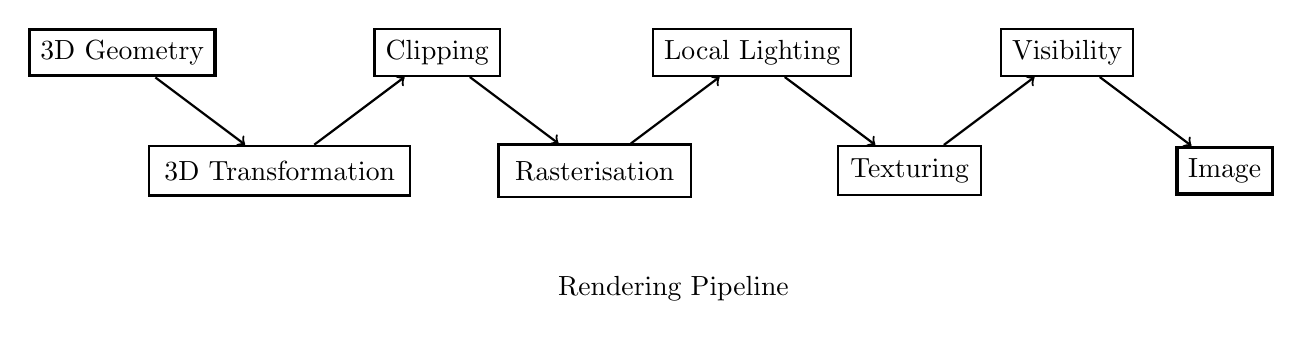
\begin{tikzpicture}{1}
\begin{scope}[every node/.style={rectangle,thick,draw, inner sep = 4pt}]
    \node [very thick] (d) at (0,0) {3D Geometry};
    \node (e) at (4,0) {Clipping};
    \node (f) at (8,0) {Local Lighting};
    \node (g) at (12,0) {Visibility};
    \node [inner sep = 5.5pt] (a) at (2,-1.5) {3D Transformation};
    \node [inner sep = 6pt] (b) at (6,-1.5) {Rasterisation};
    \node [inner sep = 4.5pt] (c) at (10,-1.5) {Texturing};
    \node [very thick] (z) at (14,-1.5) {Image};
    \node [rectangle,draw=white] (text) at (7,-3) {Rendering Pipeline};
        \path [->,thick] (d) edge (a);
        \path [->,thick] (a) edge (e);
        \path [->,thick] (e) edge (b);
        \path [->,thick] (b) edge (f);
        \path [->,thick] (f) edge (c);
        \path [->,thick] (c) edge (g);
        \path [->,thick] (g) edge (z);

\end{scope}

\end{tikzpicture}
\end{center}

\section{Representing Objects}

\begin{halfboxl}
In general, we use two different forms to represent objects, the parametric and the implicit form.

Simply speaking, we can say that a \textit{parametric function} takes in some variables and gives out a point of the object it defines.

Contrary to this, an \textit{implicit function} takes a point in space as input and returns $0$ (hence \emph{kernel}) if it lies within the object and something else if it doesn't.
\end{halfboxl}%
\begin{halfboxr}
\vspace{-\baselineskip}
\begin{defi}{Parametric Form}
An object is defined through the range of a function: $$f : D \to \mathbb{R}^3 $$
\end{defi}

\begin{defi}{Implicit Form}
An object is defined through the kernel of a function: $$f: \mathbb{R}^3 \to \mathbb{R}$$
\end{defi}
\end{halfboxr}
For the parametric form, it is easy to find all points of the object by simply plugging in all values $x \in D$. However it is difficult to determine if a certain point lies within an object.

The opposite holds for the implicit form, where checking if a point lies in an object is a simple test, but finding all points is much more difficult.

%\begin{tikzpicture}
%  \shade[ball color = gray!40, opacity = 0.4] (0,0) circle (2cm);
%  \draw (0,0) circle (2cm);
%  \fill[fill=black] (0,0) circle (1pt);
%  \draw[dashed] (0,0 ) -- node[above]{$r$} (2,0);
%\end{tikzpicture}

Consider a circle with centre $c \in \mathbb{R}^2$ and radius $r \in \mathbb{R}$.
A parametric form $f: \mathbb{R} \to \mathbb{R}^2$, that returns points on the edge of the circle, could be
\[
    f(\alpha) = \begin{pmatrix} c + cos(\alpha) \cdot r \\ c + sin(\alpha) \cdot r \end{pmatrix}
\]
To get a point lying on the edge with this formula, one just needs to plug in an angle.

But what if one wants to check whether a \emph{given} point lies on the edge? One would have to check the point against all possible results of the above formula to be sure. For that case an implicit form works a lot better:
\[
    ||p - c|| - r = 0
\]
Now to check if a point $p \in \mathbb{R}^2$ lies on the edge of the circle it can be simply plugged into the above formula.

It is clear that the choice of a representation depends on the application.


\section{Coordinate Systems}

\subsection{Extended Coordinates}

\begin{halfboxl}
To distinguish points from vectors, we can \textit{extend} the coordinates to include a fourth one. Points will have $1$ as their fourth coordinate while vectors will have $0$.

These coordinates are mathematically reasonable as the addition of two vectors and subtraction of two points yield vectors while the addition of a point and a vector yields another point. However, the addition of two points is ambiguous.
\end{halfboxl}%
\begin{halfboxr}
\vspace{-\baselineskip}
\begin{defi}{Extended Coordinates}
Using extended coordinates, the point $p = (p_1, p_2, p_3)^T \in \mathbb{R}^3$ and vector \linebreak $v = (v_1, v_2, v_3)^T \in \mathbb{R}^3$ are noted as:

$$p = \begin{pmatrix} p_1 \\ p_2 \\ p_3 \\ 1 \end{pmatrix}, \enskip v = \begin{pmatrix} v_1 \\ v_2 \\ v_3 \\ 0 \end{pmatrix} \quad p, v \in \mathbb{R}^4$$
\end{defi}
\end{halfboxr}

\subsection{Homogeneous Coordinates}
\begin{halfboxl}
\textit{Homogeneous coordinates} allow \emph{storing} dividends in the fourth component of a point by multiplying them.

Thus, divisions accumulate and in a last step called \emph{de-homogenisation} the point is divided by that fourth component. As such, divisions can be treated as \emph{multiplications}, which allows concatenating projective matrices with other matrices as explained in the following.
\end{halfboxl}%
\begin{halfboxr}
\vspace{-\baselineskip}
\begin{defi}{Homogeneous Coordinates}
With homogeneous coordinates, we represent a point $p = (p_1, p_2, p_3)^T \in \mathbb{R}^3$, for any $w \neq 0$ as follows:
$$p = \begin{pmatrix} wp_1 \\ wp_2 \\ wp_3 \\ w \end{pmatrix} \in \mathbb{R}^4$$
\end{defi}
\end{halfboxr}
\section{Mappings}

In the following section, we will be introducing mappings which we will formalise through matrices. Applying such a mapping to a point or a vector can then be written as a matrix multiplication with the matrix on the left-hand side.

Multiple mappings can be applied consecutively by multiplying them in the correct order. For example, let $M_1, \ldots , M_n \in \mathbb{R}^4$, be $n \in \mathbb{N}$ mappings and $p \in \mathbb{R}^4$ a point. Then $p'= M_n \cdot \ldots \cdot M_1 \cdot p$ is the result when applying these mappings to $p$, with $M_1$ being applied first and $M_n$ applied last. The order obviously matters, as matrix multiplication is in general not commutative.

\subsection{Linear and Affine Mappings}
\begin{halfboxl}
\vspace{-\baselineskip}
\subsubsection*{Scaling}

A scaling operation multiplies each axis by a given factor. Choosing a factor greater or smaller than $1$ results in stretching or shrinking respectively. A factor of exactly $1$ results in no change at all.

It is obvious that lengths are (generally) not preserved, and that angles are only preserved if every axis is scaled by the same factor.
\end{halfboxl}%
\begin{halfboxr}
\vspace{-\baselineskip}
\begin{defi}{Scaling}
This scaling matrix $S(\alpha, \beta, \gamma) \in R^{4\times4}$ scales the $x$, $y$ and $z$ axes by factors of $\alpha$, $\beta$ and $\gamma$ respectively:

$$S =\begin{pmatrix} \alpha & 0 & 0 & 0 \\ 0 & \beta & 0 & 0 \\ 0 & 0 & \gamma & 0 \\ 0 & 0 & 0 & 1 \end{pmatrix}$$

\end{defi}
\end{halfboxr}

\subsubsection*{Rotation}

The rotation operation is used to rotate an object around an axis. In general, any axis can be used for rotation. Though, since this is rather complex, we mostly rotate around the 3 main axes.

\begin{defi}{Rotation}
In $\mathbb{R}^3$ space we have three intuitive axes around which we can rotate, with rotation matrices \linebreak $R_x(\alpha), R_y(\alpha), R_z(\alpha) \in \mathbb{R}^4$ for an angle of $\alpha$ given as follows:


\resizebox{1\hsize}{!}{$R_x(\alpha) =
\begin{pmatrix}
1 & 0 & 0 & 0 \\
0 & \cos \alpha & -\sin \alpha & 0 \\
0 & \sin \alpha & \cos \alpha & 0 \\
0 & 0 & 0 & 1
\end{pmatrix}\;
R_y(\alpha) =
\begin{pmatrix}
\cos \alpha & 0 & \sin \alpha & 0
\\ 0 & 1 & 0 & 0
\\ -\sin \alpha & 0 & \cos \alpha & 0
\\ 0 & 0 & 0 & 1 \end{pmatrix}\;
R_z(\alpha) =
\begin{pmatrix}
\cos \alpha & -\sin \alpha  & 0 & 0
\\ \sin \alpha & \cos \alpha & 0 & 0
\\ 0 & 0 & 1 & 0
\\ 0 & 0 & 0 & 1 \end{pmatrix}$}

To rotate around an arbitrary axis $n = (n_x,n_y,n_z,1)^T, ||n|| = 1$ we use the following formula:

$$R(n,\alpha) = \cos \alpha \cdot I + (1 - \cos \alpha) \cdot nn^T - \sin \alpha \begin{pmatrix}
0 & n_z & -n_y & 0 \\ -n_z & 0 & n_x & 0 \\ n_y & -n_x & 0 & 0 \\ 0 & 0 & 0 & 1
\end{pmatrix}$$
\end{defi}

Rotation preserves lengths and angles but changes orientation and position.

\begin{halfboxl}
\vspace{-\baselineskip}
\subsubsection*{Translation}

Translating an object comes down to shifting its position by a given additive offset. This of course preserves lengths, angles and orientation, but naturally not position.
\end{halfboxl}%
\begin{halfboxr}
\vspace{-\baselineskip}
\begin{defi}{Translation}
To translate by an offset of \linebreak $t=(t_1, t_2, t_3)^T \in \mathbb{R}^3$, we write our translation matrix $T(t)\in R^{4 \times 4}$ as follows:
$$T(t)=\begin{pmatrix}
1 & 0 & 0 & t_1 \\ 0 & 1 & 0 & t_2 \\ 0 & 0 & 1 & t_3 \\ 0 & 0 & 0 & 1
\end{pmatrix}$$
\end{defi}
\end{halfboxr}

\subsection{Projective Mappings}

For the subject of projective mappings, we will be using homogeneous coordinates.

\begin{halfboxl}
\subsubsection*{Standard Projection}


The standard projection is defined by placing the camera at the origin, with the viewing vector being $(0, 0, -1)^T$ and the image plane being $z = -1$.

Projecting the point $(x, y, z, 1)^T$ using standard projection and then dehomogenizing will yield $$\big( \frac{x}{-z}, \frac{y}{-z}\big)^T.$$

\subsubsection*{Arbitrary Camera or Image Plane}

All of this being a bit boring, we can also select an arbitrary image plane, defined through $n =(n_x, n_y, n_z)^T$ and a focal distance $\delta$, while keeping our camera at the origin but pointed at the image plane.

\end{halfboxl}%
\begin{halfboxr}
\vspace{-\baselineskip}
\begin{defi}{Standard Projection}
The matrix for the standard projection looks as follows:

$$P_{std} =
\begin{pmatrix}
1 & 0 & 0 & 0 \\
0 & 1 & 0 & 0 \\
0 & 0 & 1 & 0 \\
0 & 0 & -1 & 0
\end{pmatrix}$$
\end{defi}

\begin{defi}{Arbitrary Image Plane}
For an arbitrary image plane, we have the following projection matrix:

$$P_{aip} =
\begin{pmatrix}
1 & 0 & 0 & 0 \\
0 & 1 & 0 & 0 \\
0 & 0 & 1 & 0 \\
\frac{n_x}{\delta} & \frac{n_y}{\delta} & \frac{n_z}{\delta} & 0
\end{pmatrix}$$
\end{defi}
\end{halfboxr}


We can also do the opposite by picking an arbitrary camera position, keeping the image plane passing through the origin and perpendicular to the viewing vector.

All of these projections can be deduced mathematically, but we're not going to do this here.

\begin{defi}{Arbitrary Camera Position}
The corresponding projection matrix for an arbitrary camera position with a focal distance of $\delta$ and a position $n$ is given by:$$p_{acp} =
\begin{pmatrix}
1-n_x^2 & -n_xn_y & -n_xn_z & 0 \\
-n_xn_y & 1-n_y^2 & -n_yn_z & 0 \\
-n_xn_z & -n_yn_z & 1-n_z^2 & 0 \\
\frac{n_x}{\delta} & \frac{n_y}{\delta} & \frac{n_z}{\delta} & 1
\end{pmatrix}$$
\end{defi}

\subsection{Vanishing Points}
Due to perspective foreshortening, parallel lines can meet at a certain distant point, the \emph{vanishing point}. You can observe this in nature: Take for example train rails that run parallel. When you look down the tracks you will notice that the two rails, although actually apart, meet at the horizon.
%The same applies for lovers that walk down a road towards the sunset.

To find a line's vanishing point on the image plane, we can simply intersect the line with the image plane, starting from the viewer's position. All other lines that are parallel to this line will, at infinity, appear at the same position. Also, lines that run parallel to the image plane do not have a vanishing point.

Why is that? Let's have a look at a line in explicit representation: $L(\lambda) = (x, y, z)^T + \lambda \cdot (d_x, d_y, d_z)^T$. When applying the standard projection from earlier we get $$P_{std} (L(\lambda)) = \begin{pmatrix} \frac{x + \lambda d_x}{-z - \lambda d_z} & \frac{y + \lambda d_y}{-z  - \lambda d_z} \end{pmatrix}^T.$$
In case $d_z = 0$, which means that the line runs \emph{parallel to the image plane}, $\lim_{\lambda \to \infty} P_{std} (L(\lambda)) = \infty$, which we interpret as the lack of a vanishing point.

However, when $d_z \neq 0$, then $\lim_{\lambda \to \infty} P_{std} (L(\lambda)) = \begin{pmatrix} \frac{d_x}{-d_z} & \frac{d_y}{-d_z}\end{pmatrix}$ is the vanishing point of that line. So apparently the position of the vanishing point of a line depends on its \emph{direction only}, not its position, thus all parallel lines share the same vanishing point.


\begin{halfboxl}
\vspace{-\baselineskip}
\subsection{Camera Model}

\subsubsection*{Look-At Transformation}

The first of our three transformations is the \emph{look-at transformation} which performs a basis change such that the camera is located at the origin and set up as the standard projection.
\end{halfboxl}%
\begin{halfboxr}
\vspace{-\baselineskip}
\begin{defi}{Look-At Transformation}
Given a camera position of $c$ and orthonormalised direction, up and right vectors $d$, $u$ and $r$, the look-at transformation comes down to applying the following matrix to the scene:

$$M_{LookAt} = \begin{pmatrix}
r_x & r_y & r_z & -r^Tc \\
u_x & u_y & u_z & -u^Tc \\
-d_x & -d_y & -d_z & d^Tc \\
0 & 0 & 0 & 1
\end{pmatrix}$$

\end{defi}
\end{halfboxr}

\begin{algo}{Look-At Transformation}
\textbf{Input:} Camera position $c$, direction and up vectors $d$ and $u$. \\
\textbf{Output:} A frustum-able scene with the camera in standard projection setup.
\tcblower
\begin{enumerate}
    \item Generate \emph{right} vector $r = d \times u$ as the cross product of $d$ and $u$.
    \item Calculate new \emph{up} vector $u = d \times r$.
    \item Normalise $d$, $u$ and $r$.
    \item Translate the whole scene by $-c$. The camera is now at $(0, 0, 0, 1)^T$.
    \item Rotate the scene such that $d = (0, 0, -1, 0)^T$.
    \item Rotate the scene such that $u = (0, 1, 0, 0)^T$ and $r = (1, 0, 0, 0)^T$.
\end{enumerate}
\end{algo}

\subsubsection*{Frustum Transformation}

\begin{halfboxl}
The \emph{frustum transformation} is the second one. After having defined a viewing frustum, the transformation compresses it into the $[-1,1]^3$ cube.

Such a viewing frustum can be thought of as a pyramid with its top at the camera, truncated by a near plane at the top and a far plane at the bottom, both orthogonal to the $z$-axis.

It is defined by the coordinates of its top, bottom, left and right edges on the near plane, or $t$, $b$, $l$ and $r$ respectively.

\end{halfboxl}%
\begin{halfboxr}
\vspace{-\baselineskip}
\begin{defi}{Frustum Transformation}
Given a viewing frustum with far plane $z = -f$, near plane $z = -n \ge -f$ and left, right, top and bottom coordinates $l$, $r$, $t$ and $b$, the frustum transformation is applied to a scene with the following matrix:
$$M_{Frustum} = \begin{pmatrix}
\frac{2n}{r-l} & 0 & \frac{r+l}{r-l} & 0 \\
0 & \frac{2n}{t-b} & \frac{t+b}{t-b} & 0 \\
0 & 0 & \frac{-f-n}{f-n} & -\frac{2fn}{f-n} \\
0 & 0 & -1 & 0
\end{pmatrix}$$
\end{defi}
\end{halfboxr}

\begin{center}
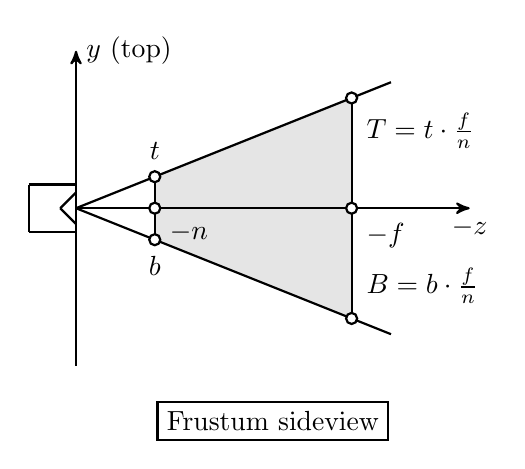
\begin{tikzpicture}[
    thick,
    >=stealth',
    dot/.style = {
      draw,
      fill = white,
      circle,
      inner sep = 0pt,
      minimum size = 4pt
    }
  ]
  \coordinate (O) at (0,0);

  \path[fill=gray!20] (1,0.4) -- (3.5,1.4) -- (3.5,-1.4) -- (1,-0.4);


  \draw[->] (0,0) -- (5,0) coordinate[label = {below:$-z$}] (xmax);
  \draw[->] (0,-2) -- (0,2) coordinate[label = {right:$y$ (top)}] (ymax);

  \draw(0,-0.3) -- (-0.6,-0.3);
  \draw(-0.6,-0.3) -- (-0.6,0.3);
  \draw(-0.6,0.3) -- (0,0.3);

  \draw[name path=n] (1,-0.4) -- (1,0.4);
  \draw[name path=f] (3.5,-1.4) -- (3.5,1.4);

  \draw(0,0) -- (4,1.6);
  \draw(0,0) -- (4,-1.6);

  \draw (1,0.4) node[dot, label= {above:$t$}] {};
  \draw (1,-0.4) node[dot, label= {below:$b$}] {};
  \draw (3.5,1.4) node[dot, label= {below right:$T = t\cdot\frac{f}{n}$}] {};
  \draw (3.5,-1.4) node[dot, label= {above right:$B = b\cdot\frac{f}{n}$}] {};

  \draw(0,0.2) -- (-0.2,0);
  \draw(0,-0.2) -- (-0.2,0);

  \draw (1,0) node[dot, label= {below right:$-n$}] {};
  \draw (3.5,0) node[dot, label= {below right:$-f$}] {};

  \draw (2.5,-2.7) node[rectangle, draw] {Frustum sideview};

\end{tikzpicture}
\begin{minipage}{.05\textwidth}
\begin{center}

\end{center}
\end{minipage}
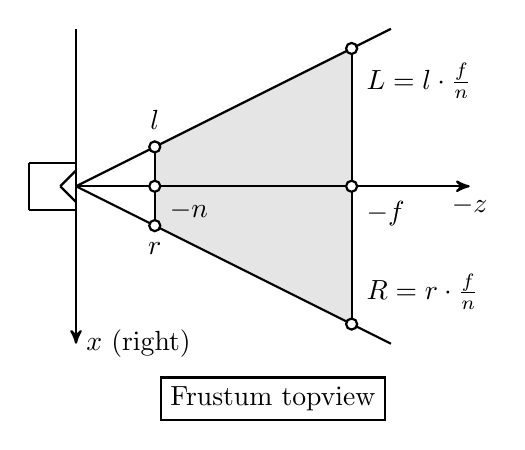
\begin{tikzpicture}[
    thick,
    >=stealth',
    dot/.style = {
      draw,
      fill = white,
      circle,
      inner sep = 0pt,
      minimum size = 4pt
    }
  ]
  \coordinate (O) at (0,0);

  \path[fill=gray!20] (1,0.5) -- (3.5,1.75) -- (3.5,-1.75) -- (1,-0.5);


  \draw[->] (0,0) -- (5,0) coordinate[label = {below:$-z$}] (xmax);
  \draw[->] (0,2) -- (0,-2) coordinate[label = {right:$x$ (right)}] (ymax);

  \draw(0,-0.3) -- (-0.6,-0.3);
  \draw(-0.6,-0.3) -- (-0.6,0.3);
  \draw(-0.6,0.3) -- (0,0.3);

  \draw[name path=n] (1,-0.5) -- (1,0.5);
  \draw[name path=f] (3.5,-1.75) -- (3.5,1.75);

  \draw(0,0) -- (4,2);
  \draw(0,0) -- (4,-2);

  \draw (1,0.5) node[dot, label= {above:$l$}] {};
  \draw (1,-0.5) node[dot, label= {below:$r$}] {};
  \draw (3.5,1.75) node[dot, label= {below right:$L = l\cdot\frac{f}{n}$}] {};
  \draw (3.5,-1.75) node[dot, label= {above right:$R = r\cdot\frac{f}{n}$}] {};

  \draw(0,0.2) -- (-0.2,0);
  \draw(0,-0.2) -- (-0.2,0);

  \draw (1,0) node[dot, label= {below right:$-n$}] {};
  \draw (3.5,0) node[dot, label= {below right:$-f$}] {};

  \draw (2.5,-2.7) node[rectangle, draw] {Frustum topview};

\end{tikzpicture}
\end{center}

\subsubsection*{Viewport Transformation}

\begin{halfboxl}
To get the scene from the cube to our screen we apply a parallel projection in which we simply neglect the $z$-coordinate. Our image now has coordinates $[-1, 1]^2$. But a screens aspect ratio is usually different from $1:1$, for example $16:9$, so to display the image we have to \emph{scale} it and \emph{add an offset} by applying the \emph{window-to-viewport} map.

After de-homogenisation, this gives us homogeneous coordinates which represent screen coordinates.
\end{halfboxl}%
\begin{halfboxr}
\vspace{-\baselineskip}
\begin{defi}{Viewport Transformation}
Given a screen width $w$ and height $h$, the viewport transformation can be applied as the following matrix:

$$M_{viewport} = \begin{pmatrix}
\frac{w}{2} & 0 & 0 & \frac{w}{2} + l \\
0 & \frac{h}{2} & 0 & \frac{h}{2} + b \\
0 & 0 & 0 & 1
\end{pmatrix}$$
\end{defi}
\end{halfboxr}

\section{Clipping}

\subsection{Line Clipping}

\subsubsection*{Cohen-Sutherland Algorithm}

\begin{halfboxl}
The \emph{Cohen-Sutherland algorithm} uses \emph{outcodes}. An outcode, defined for a point, consists of 4 bits, one for each border of the bounding box, ordered like this: top, bottom, right, left (TBRL).

If a point lies beyond a certain border line the corresponding bit is activated, as shown in the diagram.

For a line segment there are two points through which we can test if it is fully contained or fully outside in the box.
\end{halfboxl}%
\begin{halfboxr}
\vspace{-\baselineskip}
\begin{center}
    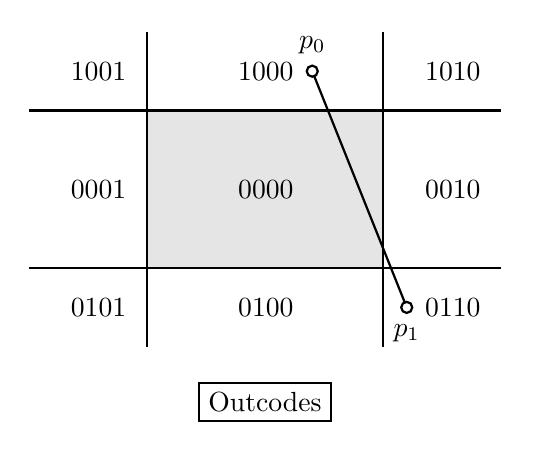
\begin{tikzpicture}[
    thick,
    >=stealth',
    dot/.style = {
      draw,
      fill = white,
      circle,
      inner sep = 0pt,
      minimum size = 4pt
    }
  ]
  \coordinate (O) at (0,0);

  \path[fill=gray!20] (1.5,-1) -- (1.5,1) -- (4.5,1) -- (4.5,-1);

  \draw(0,-1) -- (6,-1);
  \draw(0,1) -- (6,1);
  \draw(1.5,-2) -- (1.5,2);
  \draw(4.5,-2) -- (4.5,2);

  \draw (1.5,0) node[label= {left:$0001$}] {};
  \draw (1.5,1.5) node[label= {left:$1001$}] {};
  \draw (1.5,-1.5) node[label= {left:$0101$}] {};
  \draw (3.625,0) node[label= {left:$0000$}] {};
  \draw (3.625,1.5) node[label= {left:$1000$}] {};
  \draw (3.625,-1.5) node[label= {left:$0100$}] {};
  \draw (6,0) node[label= {left:$0010$}] {};
  \draw (6,1.5) node[label= {left:$1010$}] {};
  \draw (6,-1.5) node[label= {left:$0110$}] {};

  \draw (4.8,-1.5) -- (3.6, 1.5);
  \draw (4.8,-1.5) node[dot,label={below:{$p_1$}}] {};
  \draw (3.6,1.5) node[dot,label={above:{$p_0$}}] {};



  \draw (3,-2.7) node[rectangle, draw] {Outcodes};

\end{tikzpicture}
\end{center}
\end{halfboxr}

If two outcodes fulfil $(o_1 \land o_2) \neq 0$, then their line lies completely beyond at least one border, thus it is rejected. If $(o_1 \lor o_2) = 0$, then their line is completely contained in the bounding box.

If neither is fulfilled, the line may or may not be partially contained in the bounding box and while it would be possible to determine this with this algorithm, it is computationally expensive.

\subsubsection*{The Liang-Barsky Algorithm}

\begin{halfboxl}
The \emph{Liang-Barsky algorithm} uses the parametric representation of a line segment between $p_0$ and $p_1$: $$L(\lambda) = (1 - \lambda)p_0 + \lambda p_1, \quad \lambda \in [0,1].$$

For each boundary line it calculates the parameter $\lambda'$ at which the line crosses it and updates the boundaries of the line. Then, if the point enters a boundary, we use $\lambda'$ to update $\lambda_0$, else we update $\lambda_1$.
\end{halfboxl}%
\begin{halfboxr}
\vspace{-\baselineskip}
\begin{center}
    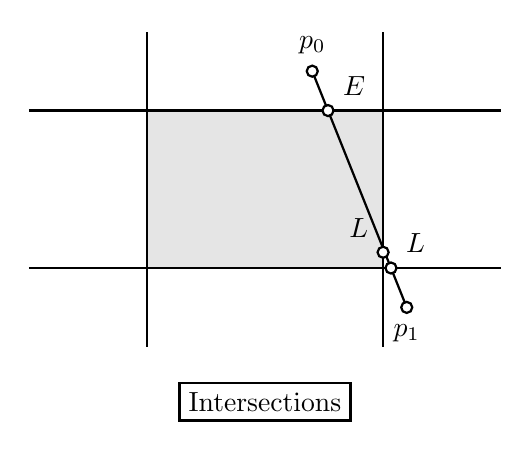
\begin{tikzpicture}[
    thick,
    >=stealth',
    dot/.style = {
      draw,
      fill = white,
      circle,
      inner sep = 0pt,
      minimum size = 4pt
    }
  ]
  \coordinate (O) at (0,0);

  \path[fill=gray!20] (1.5,-1) -- (1.5,1) -- (4.5,1) -- (4.5,-1);

  \draw(0,-1) -- (6,-1);
  \draw(0,1) -- (6,1);
  \draw(1.5,-2) -- (1.5,2);
  \draw(4.5,-2) -- (4.5,2);

  \draw (4.8,-1.5) -- (3.6, 1.5);
  \draw (4.8,-1.5) node[dot,label={below:{$p_1$}}] {};
  \draw (3.6,1.5) node[dot,label={above:{$p_0$}}] {};

  \draw (4.6,-1) node[dot,label={above right:{$L$}}] {};
  \draw (4.5,-0.8) node[dot,label={above left:{$L$}}] {};
  \draw (3.8,1) node[dot,label={above right:{$E$}}] {};


  \draw (3,-2.7) node[rectangle, draw] {Intersections};

\end{tikzpicture}
\end{center}
\end{halfboxr}

The entry test is done by calculating the direction $d = p_1 - p_0$, then calculating $n^Td$, $n$ being the boundary's normal vector. If it's negative, it's entering the boundary, else it's exiting it.

In the end, we obtain a parameter boundary $\lambda \in [\lambda_0,\lambda_1]$. If $\lambda_0 \le \lambda_1$, the line intersects the box and we render the segment, else we don't.

\subsection{Polygon Clipping}

\subsubsection*{Sutherland-Hodgman Algorithm}

\begin{halfboxl}
The \emph{Sutherland-Hodgman algorithm} is an extension of the Cohen-Sutherland algorithm. What it does is reducing clipping against the whole rectangle to clipping against boundary after boundary. For each boundary it clips every edge of the polygon, with four possible outputs.

This is done through a pipeline: the output of the first boundary is fed into the second etc.
\end{halfboxl}%
\begin{halfboxr}
\begin{itemize}
    \item \emph{Inside (the current boundary)}: we return the edge between both vertices.
    \item \emph{Outside (the current boundary)}: we return nothing.
    \item \emph{Leaving}: we return the edge between the first vertex and the intersection.
    \item \emph{Entering}: we return the edge between the intersection and the second vertex.
\end{itemize}
\end{halfboxr}

\subsubsection*{Liang-Barsky Algorithm}

The Liang-Barsky algorithm for polygons is just an extension of the line version. It first clips each edge of the polygon and then, if necessary, inserts further edges between the boundary intersections and, further, if clipping takes place around the corners, also new vertices in the corners.

\section{Rasterisation}

\subsection{Line Rasterisation}

\begin{halfboxl}
We recall the parametric and implicit representations of a line given by its endpoints $(x_0,y_0)^T$ and $(x_1,y_1)^T$.

Further, we limit our lines to slopes in $[0,1]$, as all other slopes can easily be mirrored.

\end{halfboxl}%
\begin{halfboxr}
\vspace{-\baselineskip}
\begin{align*}
    y = mx + t, & \quad m = \frac{\Delta y}{\Delta x}, \quad t = y_0 - mx_0  \\
    & ax + by + c = 0 \\
    \quad a = \Delta y, & \quad b =-\Delta x, \quad c = \Delta x t
\end{align*}
\end{halfboxr}


\begin{halfboxl}
\vspace{-\baselineskip}
\subsubsection*{Digital Differential Analysis}

\emph{Digital Differential Analysis} (DDA) calculates pixel coordinates by incremental addition and subsequent rounding of $y$.

This is better than calculating $y$ by multiplication of $x$, but is still computationally costly as we still have to round $y$.
\end{halfboxl}%
\begin{halfboxr}
\vspace{-\baselineskip}
\begin{algo}{DDA}
\textbf{Input:} A line given by its endpoints $(x_0,y_0) \text{ and } (x_1,y_1)$. \\
\textbf{Output:} None. (though it activates pixels)
\tcblower
\begin{enumerate}
    \item While $x \le x_1$:
    \item   \begin{enumerate}
                \item $x := x + 1, \quad y := \lfloor y + m \rceil$.
                \item \text{setPixel}($x$, $y$).
            \end{enumerate}
\end{enumerate}
\end{algo}
\end{halfboxr}

\begin{halfboxl}
\vspace{-\baselineskip}
\subsubsection*{The Bresenham Midpoint Algorithm}



\begin{minipage}{0.77\textwidth}
Since our slopes are restricted to $[0,1]$, the next pixel of the slope can be either \emph{East} or \emph{North East}.
\end{minipage}%
\begin{minipage}{0.03\textwidth}
\begin{center}

\end{center}
\end{minipage}%
\begin{minipage}{0.2\textwidth}
\begin{center}
    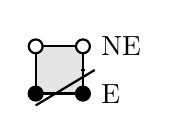
\begin{tikzpicture}[scale=0.3,
    thick,
    >=stealth',
    dot/.style = {
      draw,
      fill = white,
      circle,
      inner sep = 0pt,
      minimum size = 5pt
    }
  ]
  \coordinate (O) at (0,0);

  \path[fill=gray!20] (1,-1) -- (1,1) -- (-1,1) -- (-1,-1);

  \draw(1,-1) -- (1,1);
  \draw(1,1) -- (-1,1);
  \draw(-1,1) -- (-1,-1);
  \draw(-1,-1) -- (1,-1);

  \draw (1,1) node[dot,label={right:NE}] {};
  \draw (-1,1) node[dot] {};
  \draw (1,-1) node[dot,fill=black,label={right:E}] {};
  \draw (-1,-1) node[dot,fill=black] {};
  \draw (0.9,0) -- (1.1, 0);
  \draw (-1,-1.5) -- (1.5, 0);
\end{tikzpicture}
\end{center}
\end{minipage}

Thus, we choose to activate either E $(x_i + 1, y_i)$ or NE $(x_i + 1, y_i + 1)$ by checking if the line passes above or below the midpoint $M = \frac{\text{E } + \text{ NE}}{2}$.

We do this by simply evaluating for the implicit representation $M$ $F(M) = F(x_i + 1, y_i + \frac{1}{2})$. This is positive if we are below, and negative if we are above the line.


\end{halfboxl}%
\begin{halfboxr}
\vspace{-\baselineskip}

\begin{algo}{Bresenham Midpoint Algorithm}
\textbf{Input:} A line given by its endpoints $(x_0,y_0) \text{ and } (x_1,y_1)$. \\
\textbf{Output:} None. (though it activates pixels)
\tcblower
\begin{enumerate}
    \item $a := y_1 - y_0, \enskip b := x_0 - x_1, \enskip d := 2a + b$,
    \item $\Delta \text{E} := 2a, \enskip \Delta \text{NE} := 2(a + b)$
    \item While $x \le x_1$:
    \item \begin{enumerate}
        \item \text{setPixel}($x$, $y$), $x := x + 1$
        \item If $d \le 0: \enskip d += \Delta \text{E}$
        \item Else: $d = d + \Delta \text{NE}, \enskip y := y + 1$
    \end{enumerate}
    \item \text{setPixel}($x$, $y$)
\end{enumerate}
\end{algo}
\end{halfboxr}

But calculating $F(M)$ for each step is costly. So, we save the variable $d = F(M) = a + \frac{b}{2}$ and increment it with each step.

\vspace{10pt}

\begin{halfboxl}
Then, if E is chosen we update as follows:
\begin{align*}
    d &= F(x_i + 2, y_i + \frac{1}{2}) \\
      &= F(x_i + 1, y_i + \frac{1}{2}) + a \\
      &= d + a \\
\end{align*}
\end{halfboxl}%
\begin{halfboxr}
\vspace{-\baselineskip}
If NE is chosen, we update like this:
\begin{align*}
    d &= F(x_i + 2, y_i + \frac{3}{2}) \\
      &= F(x_i + 1, y_i + \frac{1}{2}) + a + b \\
      &= d + a + b\\
\end{align*}
\end{halfboxr}
In real life, we multiply everything by $2$ so that we can do our calculations using only integers.

\subsection{Polygon Rasterisation}

\subsubsection*{Scanline Conversion}


\begin{halfboxl}
\emph{Scanline conversion} is pretty straightforward. After sorting our polygons by their highest value $y$-points, we traverse all scanlines (horizontal pixel lines) and check for intersection with these polygons.

While doing this, we compute the fill inside the polygons by sorting the intersection points and filling the spans between odd and even intersections. But we have to cover some edge cases.
\end{halfboxl}%
\begin{halfboxr}
\vspace{-\baselineskip}
\begin{center}
    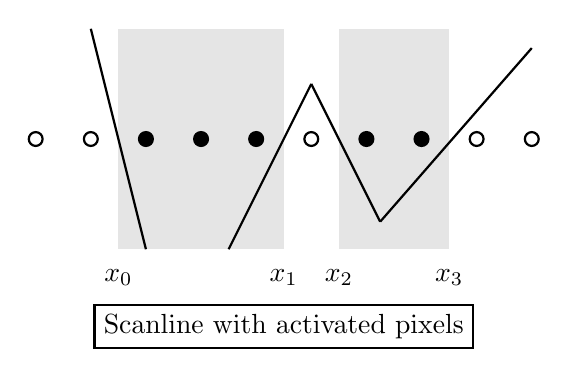
\begin{tikzpicture}[scale=1.4,
    thick,
    >=stealth',
    dot/.style = {
      draw,
      fill = white,
      circle,
      inner sep = 0pt,
      minimum size = 5pt
    }
  ]
  \coordinate (O) at (0,0);

  \path[fill=gray!20] (0.75,-1) -- (0.75,1) -- (2.25,1) -- (2.25,-1);
  \path[fill=gray!20] (2.75,-1) -- (2.75,1) -- (3.75,1) -- (3.75,-1);

  \draw (0,0)   node[dot] {};
  \draw (.5,0)  node[dot] {};
  \draw (1,0)   node[dot,fill=black] {};
  \draw (1.5,0) node[dot,fill=black] {};
  \draw (2,0)   node[dot,fill=black] {};
  \draw (2.5,0) node[dot] {};
  \draw (3,0)   node[dot,fill=black] {};
  \draw (3.5,0) node[dot,fill=black] {};
  \draw (4,0)   node[dot] {};
  \draw (4.5,0) node[dot] {};

  \draw (0.75,-1)   node[label={below:$x_0$}] {};
  \draw (2.25,-1)   node[label={below:$x_1$}] {};
  \draw (2.75,-1)   node[label={below:$x_2$}] {};
  \draw (3.75,-1)   node[label={below:$x_3$}] {};


  \draw (0.5,1) -- (1, -1);
  \draw (1.75,-1) -- (2.5, 0.5);
  \draw (2.5, 0.5) -- (3.125, -.75);
  \draw (3.125, -.75) -- (4.5, .825);

  \draw (2.25,-1.7) node[rectangle, draw] {Scanline with activated pixels};
\end{tikzpicture}
\end{center}

\end{halfboxr}


\begin{halfboxl}
We have to set horizontal spans to be half-open on the right, so that polygons with a common edge do not overlap or form gaps.

Similarly, we have to define vertices to be half-open at the top, which leads to two intersections if it is a bottom-end, none if it is a top-end and one if it is a side end.

Horizontal edges, although possibly crossing scanlines in an infinity of points, are covered the the half-openness of edges and thus generate no points.
\end{halfboxl}%
\begin{halfboxr}
\vspace{-\baselineskip}

\begin{center}
    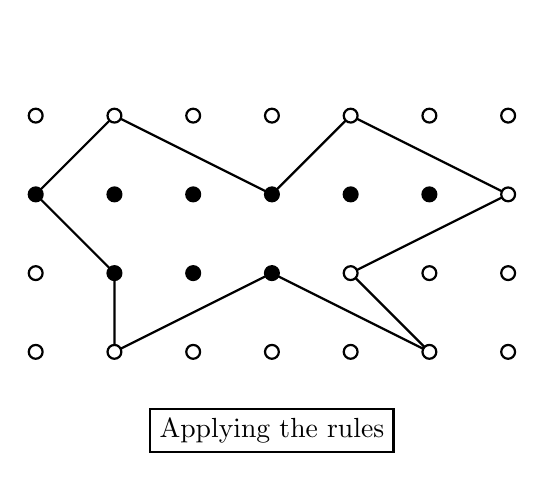
\begin{tikzpicture}[
    thick,
    >=stealth',
    dot/.style = {
      draw,
      fill = white,
      circle,
      inner sep = 0pt,
      minimum size = 5pt
    }
  ]
  \coordinate (O) at (0,0);

  \draw (1,0) -- (1,1) -- (0, 2) -- (1,3) -- (3,2) -- (4,3) -- (6,2) -- (4,1) -- (5,0) -- (3,1) -- (1,0);

  \draw (0,0)   node[dot] {};
  \draw (1,0)  node[dot] {};
  \draw (2,0)   node[dot] {};
  \draw (3,0) node[dot] {};
  \draw (4,0)   node[dot] {};
  \draw (5,0) node[dot] {};
  \draw (6,0) node[dot] {};

  \draw (0,1)   node[dot] {};
  \draw (1,1)  node[dot,fill=black] {};
  \draw (2,1)   node[dot,fill=black] {};
  \draw (3,1) node[dot,fill=black] {};
  \draw (4,1)   node[dot] {};
  \draw (5,1) node[dot] {};
  \draw (6,1) node[dot] {};

  \draw (0,2)   node[dot,fill=black] {};
  \draw (1,2)  node[dot,fill=black] {};
  \draw (2,2)   node[dot,fill=black] {};
  \draw (3,2) node[dot,fill=black] {};
  \draw (4,2)   node[dot,fill=black] {};
  \draw (5,2) node[dot,fill=black] {};
  \draw (6,2) node[dot] {};

  \draw (0,3)   node[dot] {};
  \draw (1,3)  node[dot] {};
  \draw (2,3)   node[dot] {};
  \draw (3,3) node[dot] {};
  \draw (4,3)   node[dot] {};
  \draw (5,3) node[dot] {};
  \draw (6,3) node[dot] {};

  \draw (6,4) node[] {};


  \draw (3,-1) node[rectangle, draw] {Applying the rules};
\end{tikzpicture}
\end{center}
\end{halfboxr}

For this algorithm to be efficient, we need to apply a few further tricks. So, for each edge, we determine if they cross the current scanline by comparing their $y$-span to the the scanline. For this, we keep two ordered, appropriately named lists, the \emph{passive} and the \emph{active list}, which are sorted by $y_{min}$ and $y_{max}$ respectively.

The active list is empty at the beginning, and once we enter the scanline $y + 1$, we shift all edges with $y_{min} = y + 1$ from the passive to the active list. They are then discarded once $y_{max} \le y + 1$.

\subsubsection*{Pineda Method}

To rasterise \textbf{convex} polygons, we use the \emph{Pineda method}. We take a list of its counterclockwise vertices $v_0,\ldots,v_n$ and define its edges $E_i, \enskip 1 \le i \le n$ correspondingly. $F_i(x,y)$ being the implicit representation of such an edge, we compute, for any pixel candidate $(x,y)$, the tuple $(F_1(x,y),\ldots,F_n(x,y))$.
This pixel will be inside this polygon iff, $\Forall i \in \Set{1,\ldots,n}: \enskip F_i(x,y) \le 0$.


\subsection{Triangulation}

\subsubsection*{Marching (Corner Cutting)}

Conceptually, Corner Cutting is about taking a polygon, selecting a vertex, creating a triangle with its neighbours and removing it until only one triangle is left. The difficulty lies in is choosing a triangle that is actually \emph{completely inside} the polygon.

First, we need to select a convex corner. Given the triangle $\Delta(p_{i-1},p_i,p{i+1})$, this can be determined by the sign of the cross product $(p_{i-1} - p_i) \times (p_{i+1} - p_i)$. Which sign it needs is determined by the point with the lowest $x$-coordinate, since its triangle \textbf{must} be convex.

We must also check that no vertex lies within the triangle we want to cut of, so we check that, too, for each vertex, or better, only for the concave vertices.

\subsubsection*{Delaunay Triangulation}

\begin{halfboxl}
A very nice form of triangulation is the \emph{Delaunay Triangulation}. Its main characteristic is that, for any triangle, the respective circumcircle does not contain any other point. This leads to a very regular triangulation.

The algorithm to create such a triangulation uses three operations to achieve this:
\begin{itemize}
    \item \emph{1-3 Split}: A vertex that lies strictly within a triangle is connected to the three vertices.
    \item \emph{2-4 Split}: A vertex that lies on the edge between two triangles destroys that edge and is connected to all four nodes.
    \item \emph{Edge Flip}: Given two triangles sharing an edge, if the circumcircle of one of the triangles contains the remaining point of the other triangle, that shared edge is flipped to connect the two vertices that weren't connected.
\end{itemize}

\end{halfboxl}%
\begin{halfboxr}
\vspace{-\baselineskip}
\begin{algo}{Delaunay Triangulation}
\textbf{Input:} A set of points $\Set{p_1,...,p_n}$. \\
\textbf{Output:} A Delaunay Triangulation of the point set.
\tcblower
\begin{enumerate}
    \item Add three further points around the point cloud of $p_1,...,p_n$ and create edges between them.
    \item For each point from the set: \begin{enumerate}
        \item If it lies within a triangle, perform a 1-3 Split.
        \item If it lies within a tron the edge of two triangles, perform a 2-4 Split.
        \item Restore the Delaunay property with Edge Flips.
    \end{enumerate}
  \item Finally, delete the three points and corresponding edges and faces that were added in the first step.
\end{enumerate}
\end{algo}
\end{halfboxr}

\subsection{Voronoi Diagram}

A \emph{Voronoi Diagram} is the dual mesh to a Delaunay triangulation. What it does is splitting the space into Voronoi regions. Given a set of points, the Voronoi region of a point is the \emph{convex} area around it to which it is the closest vertex.

\subsubsection*{Sweepline}

\begin{halfboxl}
The sweepline algorithm generates a Voronoi diagram for a given set of points. Its main aspect is the detection of \emph{circle} and \emph{point} events.

A circle event occurs when the sweepline reaches a point where three points that have already been discovered form a circle without another point being detected.

A point event occurs when the sweepline detects a new point before such a circle can be formed.


\end{halfboxl}%
\begin{halfboxr}
\vspace{-\baselineskip}
\begin{algo}{Sweepline Algorithm}
\textbf{Input:} A set of points $\Set{p_1,...,p_n}$. \\
\textbf{Output:} A Voronoi Diagram of the point set.
\tcblower
\begin{enumerate}
    \item Sort points by $x$-coordinate.
    \item \emph{Sweep} along the $x$-axis.
    \item Detect and process point and circle events.
\end{enumerate}
\end{algo}
\end{halfboxr}


\begin{halfboxl}
\vspace{-\baselineskip}
\begin{center}
    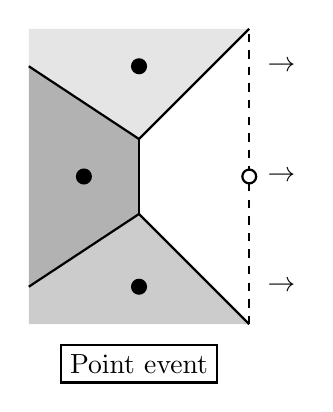
\begin{tikzpicture}[scale=1.4,
    thick,
    >=stealth',
    dot/.style = {
      draw,
      fill = white,
      circle,
      inner sep = 0pt,
      minimum size = 5pt
    }
  ]
  \coordinate (O) at (0,0);

  \path[fill=gray!20] (0,1) -- (1,.34) -- (2,1.34) -- (0,1.34);
  \path[fill=gray!40] (0,-1) -- (1,-.34) -- (2,-1.34) -- (0,-1.34);
  \path[fill=gray!60] (0,1) -- (1,.34) -- (1,-.34) -- (0,-1);


  \draw (2,-1)   node[dot,white,label={right:$\rightarrow$}] {};
  \draw (2,0)   node[dot,white,label={right:$\rightarrow$}] {};
  \draw (2,1)   node[dot,white,label={right:$\rightarrow$}] {};

  \draw [dashed] (2,-1.34) -- (2,1.34);


  \draw (1,-.34) -- (1,.34);
  \draw (0,1) -- (1,.34);
  \draw (2,1.34) -- (1,.34);
  \draw (0,-1) -- (1,-.34);
  \draw (2,-1.34) -- (1,-.34);


  \draw (0.5,0)   node[dot,fill=black] {};
  \draw (1,-1)   node[dot,fill=black] {};
  \draw (1,1)   node[dot,fill=black] {};
  \draw (2,0)   node[dot] {};



  \draw (1,-1.7) node[rectangle, draw] {Point event};
\end{tikzpicture}
\end{center}
\end{halfboxl}%
\begin{halfboxr}
\vspace{-\baselineskip}
\begin{center}
    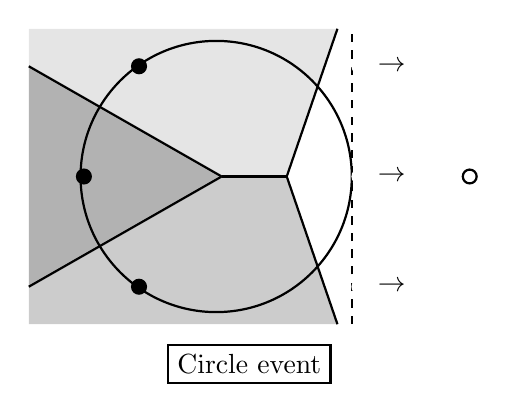
\begin{tikzpicture}[scale=1.4,
    thick,
    >=stealth',
    dot/.style = {
      draw,
      fill = white,
      circle,
      inner sep = 0pt,
      minimum size = 5pt
    }
  ]
  \coordinate (O) at (0,0);

  \path[fill=gray!20] (0,1) -- (1.75,0) -- (2.34,0) -- (2.8,1.34) -- (0,1.34);
  \path[fill=gray!40] (0,-1) -- (1.75,0) -- (2.34,0) -- (2.8,-1.34) -- (0,-1.34);
  \path[fill=gray!60] (0,1) -- (1.75,0) -- (0,-1);

  \draw [dashed] (2.93,-1.34) -- (2.93,1.34);

  \draw (0,1) -- (1.75,0);
  \draw (0,-1) -- (1.75,0);
  \draw (1.75,0) -- (2.34,0);
  \draw (2.34,0) -- (2.8,1.34);
  \draw (2.34,0) -- (2.8,-1.34);

  \draw (1.7,0) circle (35pt);

  \draw (0.5,0)   node[dot,fill=black] {};
  \draw (1,1)   node[dot,fill=black] {};
  \draw (1,-1)   node[dot,fill=black] {};
  \draw (4,0)   node[dot] {};

  \draw (3,-1)   node[dot,white,label={right:$\rightarrow$}] {};
  \draw (3,0)   node[dot,white,label={right:$\rightarrow$}] {};
  \draw (3,1)   node[dot,white,label={right:$\rightarrow$}] {};


  \draw (2,-1.7) node[rectangle, draw] {Circle event};
\end{tikzpicture}
\end{center}
\end{halfboxr}

The two diagrams above illustrate point and circle events. Note that the dashed line and the arrows symbolise the sweepline and its movement.

\section{Lighting}

\subsection{Local Lighting}

With the Phong Model, we can compute the lighting of any point $p$ of colour $\alpha$ and normal $n$, given a viewing position $v$ and light source position $l$.

\begin{halfboxl}
The material property $\alpha$ is given by a diagonal matrix $\alpha \in \mathbb{R}^{3 \times 3}$ with scalar entries $\alpha_r,\alpha_g,\alpha_b \in [0,1]$ for the red, green and blue component respectively.

The light intensities $C$ are given by three dimensional colour vectors.

On the right, we preemptively introduce the full formula used by the Phong model. In the following sections we will analyse its components.
\end{halfboxl}%
\begin{halfboxr}
\vspace{-\baselineskip}
\begin{defi}{Phong Model}
The local lighting of the Phong model is given by:
\begin{align*}
C_{orig} =  & \enskip C_a \cdot \alpha_a \\
            & \enskip + \sum_l \bigg(\text{spot}(p,l) \cdot \text{att}(p,l)\\
            & \qquad \cdot \big[C_d(p,n,l) + C_{sp}(p,n,v,l)\big]\bigg)
\end{align*}
\end{defi}
\end{halfboxr}
It can be decomposed into \emph{ambient lighting}, \emph{diffuse lighting} and \emph{specular lighting}, as well as \emph{spotlight} and \emph{attenuation effects}. We will first introduce the three different forms of lighting and then the secondary effects.


\begin{halfboxl}
\vspace{-\baselineskip}
\subsubsection*{Ambient Lighting}

Since usually no scene is completely dark, \textit{ambient lighting} independent of light source or the viewers position is determined only by surface materials and ambient light intensity.
\end{halfboxl}%
\begin{halfboxr}
\vspace{-\baselineskip}
\begin{defi}{Ambient Lighting}
Given $C_A$, the ambient light intensity, the ambient lighting is given by:
$$C_a = \alpha_a \cdot C_A$$

\end{defi}
\end{halfboxr}

\subsubsection*{Diffuse Lighting}


\begin{halfboxl}
\vspace{-\baselineskip}
\textit{Diffuse Lighting} models the reflection on matte or rough surfaces. It can also be formulated as the amount of light hitting a certain point from a certain light source.

While dependent on the material, it is also dependent on the relative position of the light source to the surface.
\end{halfboxl}%
\begin{halfboxr}
\vspace{-\baselineskip}
\begin{defi}{Diffuse Lighting}
Given a light source emitting the light $C_l$, the diffuse lighting is given by:
$$C_d(p,n,l) = \alpha_d \cdot C_l \cdot \frac{n^T \cdot (l-p)}{||l-p||}$$
\end{defi}
\end{halfboxr}

\subsubsection*{Specular Lighting}

\begin{halfboxl}
\textit{Specular lighting} models the behaviour of light on a shiny surface, off which it is reflected with the same angle with which it hit it. The outgoing vector is given by $r$. Thus, it is of course dependent on the position of the light source, but also on the position of the viewer.

We also need to take into account the \emph{shininess exponent} $s$, since there are varying degrees of shininess. The higher $s$ is, the shinier the surface, and thus the preciser the reflection is.

As the classic formula is pretty expensive to compute, it is easier to approximate it using the \emph{Phong-Blinn approximation}.
\end{halfboxl}%
\begin{halfboxr}
\vspace{-\baselineskip}
\begin{defi}{Specular Lighting}
$$C_{sp} (p,n,v,l) = \alpha_{sp} \cdot C_l \cdot \bigg(\frac{r^T(v-p)}{||r||\cdot||v-p||}\bigg)^s$$ with $$r = (2nn^T-I)(l-p)$$
\end{defi}

\begin{defi}{Phong-Blinn Approximation}
$$C_{sp}(p,n,v,l) \approx \alpha_{sp}  \cdot C_l \cdot \big(n^Th\big)^s$$ with $$h= \frac{v + l}{||v + l||}$$
\end{defi}
\end{halfboxr}
\subsubsection*{Attenuation}

\begin{halfboxl}
\vspace{-\baselineskip}


The attenuating factor for a point, given a light source, is about the distance of the point from the light source; the greater the distance between them, the weaker the reflection should be.

For a more accurate representation, we do not only consider a linear, but also a quadratic attenuation.
\end{halfboxl}%
\begin{halfboxr}
\vspace{-\baselineskip}
\begin{defi}{Attenuation}
Given linear and quadratic attenuation factors $\text{att}_{\text{lin}}$ and $\text{att}_{\text{quad}}$, the attenuation for a point and a light source is given by:

\resizebox{1\linewidth}{!}{$\text{att}(p,l) = \frac{1}{\text{att}_{\text{lin}}\cdot||p-l|| + \text{att}_{\text{quad}}\cdot||p-l||^2}$}

\end{defi}
\end{halfboxr}

\begin{halfboxl}
\vspace{-\baselineskip}
\subsubsection*{Spotlight}

If, instead of our usual light sources which emit in all directions equally, the light source at $l$ is a spotlight emitting light focused in a direction $d$ then the further we are away from this vector, the weaker the reflection will be.

The impact of that distance is given by the exponent $f$.
\end{halfboxl}%
\begin{halfboxr}
\vspace{-\baselineskip}
\begin{defi}{Spotlight}
The spotlight factor of a light source, given a direction $d$ and an exponent $f$ is defined as:
$$\text{spot}(p,l) = \bigg(\frac{d^T(p-l)}{||p-l||}\bigg)^f$$
\end{defi}
\end{halfboxr}

\begin{halfboxl}
\vspace{-\baselineskip}
\subsubsection*{Depth Cueing}

In outdoor scenes we want to be able to model the blue-gray of far away objects. This is done through depth cueing. Factoring in the distance to the viewer $b$, it overlays the colour of an object with such a filter.
\end{halfboxl}%
\begin{halfboxr}
\vspace{-\baselineskip}
\begin{defi}{Depth Cueing}
Given a blue-gray colour filter $C_{dc}$, we can model an atmosphere like this:
$$C_{final} = b \cdot C_{orig} + (1-b) \cdot C_{DC}$$
\end{defi}
\end{halfboxr}

\begin{halfboxl}
\subsection{Shading}
%The shading algorithm calculates the colour for each fragment using a lightning simulation. The lecture presents three algorithms: Flat shading, Gouraud shading and Phong shading.
Shading algorithms are applied to give the impression of depth by varying levels of darkness on objects. We take a look at three possible approaches in the following.

\subsubsection*{Gouraud shading}
Gouraud shading computes lighting values \emph{per vertex} and interpolates them over a polygon, i.e. for each fragment on the polygon, the colour values from the vertices are interpolated.

While Gouraud shading works great for shading surfaces that reflect light diffusely it may not always work great with specular light. Its shape depends on the underlying polygons and the quality of it thus depends on the number of vertices of your model. It is computationally less expensive than Phong shading though.
\end{halfboxl}%
\begin{halfboxr}
\subsubsection*{Flat shading}
%For each \emph{surface}, one colour is calculated using the Phong model. That colour is then assigned to all fragments that belong to the surface.
Flat shading computes lighting values for \emph{one vertex} per polygon and uses the resulting colour for the entire polygon, resulting in a single flat colour for every polygon. The individual polygons can be seen.

\subsubsection*{Phong shading}
%In Phong shading, for each surface the normals are interpolated. The Phong model is then used to calculate the colour for each fragment using the interpolated normals.
Not to be confused with the Phong lighting model, Phong \emph{shading} interpolates the lighting parameters across the polygon and computes the lighting \emph{per fragment}, not per vertex.

Although more computationally expensive than Gouraud shading, you get good looking, round, smooth specular highlights that move smoothly along the surface as the camera, model or light moves. No visible artefacts from the polygon edges.
\end{halfboxr}

\subsection{Shadows}

To introduce the effects of shadows, a term $S(p,l)$ is added to the lighting equation that tests if the point $p$ is in the shadow of the light source at $l$:

  $$ S(p,l) =\begin{cases}
    0, \quad \text{if the light } l \text{ is blocked at point } p, \\
    1, \quad \text{else}.
    \end{cases}$$
Then the colour can be computed as:

$$ C_{orig} =  C_a \cdot \alpha_a + \sum_l \bigg(\text{spot}(p,l) \cdot \text{att}(p,l) \cdot \text{S}(p,l) \cdot \big[C_d(p,n,l) + C_{sp}(p,n,v,l)\big]\bigg)
$$

Shadows are caused by objects blocking light. What we effectively perform are visibility tests from the perspective of the light source. We could (pre-)compute shadows based on the light and the geometry of occluding objects (occluders) or shadow textures, but this approach is usually too slow for real-time applications. Instead of using two-dimensional shapes, projected on occluded objects (occludees), we compute the \emph{three-dimensional region} that lies in the shadow of an object and light source, for example as \emph{Shadow Volumes} which are described in the following.

\subsubsection*{Shadow Volumes}

A Shadow Volume is a cone-like volume to infinity, starting at the silhouette of an object, cast by a light source. A silhouette of an object can be easily found as it is built by the edges that separate front- and back-facing polygons w.r.t. the light source. The number of shadow volumes we need to compute is $\# occluder \cdot \# lights$.

During visibility tests we raycast through each pixel of the final image into the scene onto an intersection point to find the closest polygon. We can extend this and check whether this point lies within a volume by simply counting all intersections of the ray with shadow volumes. For every volume entered or left by the ray, we increment or decrement the counter respectively. If the counter is non-zero as we reach the intersection point, it lies inside of (at least) one shadow volume.

This method fails if the camera is positioned inside a shadow volume and is referred to as \emph{$z$-fail}. To avoid this issue, we add a back-cap to each volume and instead of tracking the ray intersections with volumes \emph{in front of} $p$, we count the intersections \emph{behind} $p$, with incrementation and decrementation switched.

\subsubsection*{Shadow Maps}
By rendering the scene as seen from the position of the light source and storing the contents of the resulting Z-Buffer, we get so called Shadow Maps that store the distances between the light source and occluders.

To check whether a point $p$ lies inside of a shadow, we simply project it onto our shadow map with the model-view and projection matrix used to create the shadow map. We can now compare the depth values: If the depth of $p$ is greater than the stored value on the shadow map, the point lies behind another object and the light has no effect on its colour.

\subsubsection*{Perspective Shadow Maps}
\label{subsubsec::perspectiveShadowMaps}

\begin{halfboxl}
The resolution of the shadow map is the resolution of the depth buffer. This means that many fragments get projected onto the same pixel of the shadow map.
This effect is expressed by the formula on the right.
\end{halfboxl}
\begin{halfboxr}
\vspace{-\baselineskip}
\begin{defi}{Perspective Shadow Maps}
\begin{center}
    $h_s \cdot \frac{r_s}{r_i} \cdot \frac{cos(\beta)}{\cos(\alpha)}$
\end{center}
\end{defi}
\end{halfboxr}

The first fraction is perspective aliasing and the second projective aliasing. Calculating the shadow map using normalised device coordinates reduces the perspective aliasing to $1$. The projective aliasing can not be reduced in general.

\begin{halfboxl}
\subsubsection*{Properties of Shadow Volumes}
\begin{itemize}
    \item Precise shadows, little aliasing
    \item Works with omnidirectional lights
    \item Requires closed mesh
    \item Need to be rendered twice for each frame, no hardware support, complexity and amount of occluders can make this \emph{slow}
\end{itemize}
\end{halfboxl}%
\begin{halfboxr}
\subsubsection*{Properties of Shadow Maps}
\begin{itemize}
    \item Very general method
    \item Resource hungry
    \item Incompatible with omnidirectional lights
    \item Discrete, thus imprecise; artefacts
    \item Can be done on hardware, \emph{fast}
\end{itemize}
\end{halfboxr}

\section{Texturing}

The art of texturing is to map a 2-dimensional texture onto the surface of a mesh. This \emph{U-V-Mapping}, called this way because the texture coordinates are labelled $u$ and $v$, is a big topic. The original topic of textures was to give a model more colour detail.

In more complex materials, U-V-Mapping can project a \emph{map} onto the geometry, assigning a material property value, like the specular value, to each point on the geometry.

\subsection{Environment maps}
Using texture maps we can also precompute the approximate reflection of the environment of e.g. a sphere. All we need is a photograph of such a proxy reflecting the environment as the texture map. Now, given a \emph{normalised} direction vector $d$ of the surface, we can easily map the proper texture colour onto it:

\begin{enumerate}
    \item Add 1 to the $z$-coordinate of $d$.
    \item Normalise $d$.
    \item Use the $x$- and $y$-coordinates of $d$ to look up colour in the texture.
\end{enumerate}

\subsubsection*{Magnification \& Minification}
When projecting the scene onto the image plane using nearest-neighbour, we may face two issues:
\begin{enumerate}
    \item Magnification: many screen pixels display only few texels, so texels will appear jagged.
    \item Minification: many texels are mapped to one pixel (which can only take one colour), which results in Moiré patterns.
\end{enumerate}

A solution to this is to use \emph{bilinear interpolation} that looks up the colour interpolating multiple colours.

\subsection{Anti-Aliasing}
Aliasing are a set of effects that occur during different steps of the rendering pipeline:

\begin{itemize}
    \item \textbf{Texture alias:} For the computation of the colour of a fragment based on a texture, only one point is sampled from the texture even if an area is projected onto the fragment. This leads to moire-like patterns if the area is large and to hard edges between individual texels if the area is small.
    \item \textbf{Geometry alias:} To determine if a triangle covers a pixel, one point is sampled and a binary decision is made. This leads to jagged edges when two triangles with stark colour differences meet.
    \item \textbf{Shader alias:} If a texture creates an edge within a polygon, for example a transparent texture, the edge can have alias effects that are not corrected by anti-aliasing algorithms used for geometry alias.
    \item \hyperref[subsubsec::perspectiveShadowMaps]{\textbf{Shadow alias}}
\end{itemize}

\subsubsection*{MIP-Mapping}

The optimal solution to texture aliasing is to integrate over the area of the texture that is projected onto the fragment. This solution is very complex and slow. For ray-tracing supersampling, taking the average colour of multiple points is optimal.

For rasterisation, a good way is to use \emph{MIP-Maps} and \emph{trilinear filtering}. The texture is stored in multiple resolutions, increasing the memory by 33\%. Each resolution is called a \emph{level}. The GPU calculates the optimal level for a given fragment, the farther the texture is away, the lower is the resolution.

In the general case, the calculated level is between to existing levels and the projected position of the texture is between to texels. Therefore the colours of the two levels, and in each level between the tow texels in $u$ and $v$ direction, is interpolated. Resulting in trilinear interpolation.

\subsubsection*{Anisotropic Filtering}

Most of the time, a pixel is not projected into a perfect square on the texture. The pixel can span more texels in the $u$ than in the $v$ direction. This is alleviated by \emph{anisotropic filtering}. Multiple points in different positions on the project area are sampled using trilinear interpolation. The number and position of sampling points can be based on the angle of the sampled texture.

\subsubsection*{Full-Scene Anti-Aliasing}

The problem with geometry aliasing is that in the end only one triangle is contributing to the colour of a pixel, even if multiple triangles cover the pixel partially.

The optimal solution is to compute the size of the area that is covered by a triangle for each pixel, sample the colour and then blend the colours with a weighted manner. This is slow. Seriously, don't implement this, except if you own Nvidia stocks.

A trivial solution is to render the scene with twice the resolution and scale the image down as the last step. This approach called \emph{Full-Scene Anti-Aliasing} or FSAA uses 4 coverage samples for each pixel, and creates one fragment if at least one sample point is covered.
It then samples the colour at the same positions, that are covered and therefore creates 4 colours that are blended after the visibility test.

\subsubsection*{Multisample Anti-Aliasing}

A downside to FSAA is that the sampling positions are on a uniform gird. This creates artefacts for edges that run parallel to the image grid.
Second, for a pixel where two triangles cover halve of it, two (similar) colours a sampled for each triangle, using more computations power.

\emph{Multisample Anti-Aliasing} or MSAA uses a changeable number of coverage samples at variable positions. If the triangle covers the pixel, one fragment is created and the colour is sampled once and copied to all cover sample points, creating multiple colour values that are blended in the end of the rendering pipeline.

\subsubsection*{Coverage Sampling Anti-Aliasing}

It is rare for a pixel to be covered by more than 4 triangles. \emph{Coversampling Anti-Aliasing} or CSAA saves memory by storing up to four colours and a mapping of the colours to the cover sampling positions, instead of copying the sampled colour the corresponding sample positions. The final colours of the pixel are blended weighted by the number of positions each colour is mapped to.

\subsubsection*{Postprocessing Anti-Aliasing}

For shader aliasing, a simple solution is to use \emph{Postprocessing Anti-Aliasing} or FXAA. It detects edges after the rendering pipeline is finished and blends them. This gets rid of shader aliasing but can smooth colour edges that are meant to be sharp, for example the edge between the UI and the background in a game.

The edge detection can use information form the rendering pipeline like depth values, colour values or even the previous frame.

\section{Polygonal Meshes}

We can approximate objects using polygonal meshes. Such a mesh consists of a geometry, which defines the shape of an object through the vertices, and a topology, which specifies the edges and faces of an object. In the following, we will mainly deal with triangular meshes in $\mathbb{R}^2$ and $\mathbb{R}^3$ space and will refer to polygonal meshes simply as meshes. We will let $V$, $E$ and $F$ stand for the number of vertices, edges and faces respectively.

\subsection{Properties}

For any mesh (the \emph{primal mesh}), we define its \emph{dual mesh} as a mesh in which any $k$-dimensional entity is replaced by a $(2-k)$-dimensional one. Or, for our purposes, we replace faces by points and vice versa, and keep the vertices.

Our meshes are $2$\emph{-manifolds}, meaning that they are surfaces with no extra entities attached. Formally, they fulfil

\begin{itemize}
    \item the \emph{local disk property} (for any point, there is an $\epsilon$-ball whose intersection with the surface is homeomorphic to a disc),
    \item the \emph{edge ordering property} (edges can be uniquely ordered in a (counter-)clockwise fashion) and
    \item the \emph{face count property} (interior edges have exactly two neighbouring faces, boundary edges exactly one).
\end{itemize}

Sometimes, our meshes are \emph{closed}, that is, there are no boundary edges.

\subsection{Euler's Formula}

\begin{halfboxl}
Euler's Formula gives the relation between the number of vertices, faces, edges and the genus of an object has and is given by:

$$V - E + F = 2 (1 - g)$$

This can easily be proven by induction over the size of the mesh for planar (vertex insertion, vertex addition) and 3D meshes (face split, edge split).
\end{halfboxl}%
\begin{halfboxr}
\vspace{-\baselineskip}
\begin{defi}{Genus}
The genus of an object is given by the amount of handles attached to it. That is, a sphere has genus $0$, a donut has genus $1$ etc. It can be derived from the Euler formula:

$$g = 1 - \frac{V - E + F}{2}$$
\end{defi}
\end{halfboxr}

For triangle meshes, we can define a constant $c$ such that $c = 2(1 - g) = V - E + F$. By then splitting the edges into halfedges, we have 3 halfedges per face, thus we write, $3F = HE \Leftrightarrow 3F =2E$.

Inserting this into the Euler Formula, we have $2V - F = c$. And since normally, V and F are considerably larger than $c$, we have $F \approx 2V$. We can also derive that $HE \approx 6V$.

\subsection{Platonic Solids}

Platonic solids are convex polyhedra with the properties that they are closed, that they have genus $0$, that all faces are regular $p$-gons and and that all vertices have valence $q$.

\begin{halfboxl}
We can derive all existing platonic solids by using the Euler formula and the above properties. This is done by assigning half edges to vertices $HE = 2E = qV$ and to faces $HE = 2E = pF$ respectively. We can transform these equations, insert the results into the Euler Formula and obtain $E$, $V$ and $F$ in function of $p$ and $q$.
\end{halfboxl}%
\begin{halfboxr}
\vspace{-\baselineskip}
\begin{defi}{Schläfli-Symbol}
For a give platonic solid made of regular $p$-gons and vertex valence $q$, the Schläfli-Symbol is given by:
$$\Set{p,q}$$
\end{defi}
\end{halfboxr}

Then, as $p \ge 3$, $2p - pq +2q > 0$ and $V,E,F > 0$ must hold, we can derive all possible platonic solids. As an example, the cube, which has vertex valence $3$ and is made of squares, is given by the Schläfli-Symbol $\Set{4,3}$. Additionally, a solid with Schläfli-Symbol $\Set{m,n}$ is dual to the solid with symbol $\Set{n,m}$.

\subsection{Datastructures}

\begin{halfboxl}
\vspace{-\baselineskip}

\subsubsection*{Triangle Lists}

A possibility would be to simply store any triangle by specifying its three vertices.

\subsubsection*{Shared Vertex}

We can reduce the redundancy by saving a list of vertices and their coordinates on one hand and a list of triangles made of said vertices on the other. This is the principle of the \emph{shared vertex} technique.

\end{halfboxl}
\begin{halfboxr}
\vspace{-\baselineskip}

\subsubsection*{Triangle Strips}

This redundance can be further reduced if instead of saving the topology separately, we implicitly saved it through ordering of the vertices. This construct is called a \emph{triangle strip}. In practice, we require more than one of these strips to describe the topology.

\subsubsection*{Triangle Fans}

The idea of triangle fans is to save faces sharing a central vertex. For $N$ faces, we save $N+2$ edges.
\end{halfboxr}







\subsubsection*{Edge Based Structure}

\begin{halfboxl}
The \emph{Winged Edge} datastructure saves, for vertices and faces, pointers to an incident edge each, and for each edge pointers to its two vertices.

Further to that, it stores four edge pointers, two for each incident vertex, of which one is oriented clockwise, the other counterclockwise. Finally, it also stores one pointer for each incident face.
\end{halfboxl}%
\begin{halfboxr}
\vspace{-\baselineskip}
\begin{defi}{Winged Edge Structure}
The Winged Edge structure saves, for each edge, vertex and face, the following data:
$$e = [^*v_0,^*v_1,^*e_{0c},^*e_{0cc},^*e_{1c},^*e_{1cc},^*f_0,^*f_1]$$
$$v=[^*e], \quad f=[^*e]$$
\end{defi}
\end{halfboxr}

\begin{halfboxl}
\subsubsection*{Face Based Structures}

This structure is impractical since in trying to jump along the faces around one vertex, we need to check which face we came from to continue in the right direction. Further, we do not actually save the edges, thus they are not represented.
\end{halfboxl}%
\begin{halfboxr}
\vspace{-\baselineskip}
\begin{defi}{Face Based Structure}
In a face based structure, for each face, we save pointers to its vertices and its neighbouring faces, and a pointer to one face for each vertex:
$$f=[^*v_0,^*v_1,^*v_2,^*f_0,^*f_1,^*f_2] \quad v = [^*f]$$
\end{defi}
\end{halfboxr}




\begin{halfboxl}
\subsubsection*{Halfedge Based Structure}

Here, we replace and edge $v_0 v_1$ by two halfedges $\overrightarrow{v_0 v_1}$ and $\overrightarrow{v_1 v_0}$.For each such halfedge, we store four pointers, one to its opposite halfedge, one to its succeeding halfedge, one to the vertex it points to and one to its incident face.
\end{halfboxl}%
\begin{halfboxr}
\vspace{-\baselineskip}
\begin{defi}{Halfedge Based Structure}
For a halfedge $h$, we save $$h = [^*h_{opp},^*v,^*f,^*h_{next}].$$
For a vertex $v$ and a face $f$ we store $$v = [^*h], \quad f = [^*h]$$
\end{defi}
\end{halfboxr}

\subsubsection*{Valence Coding}

\begin{halfboxl}
\vspace{-\baselineskip}
\begin{algo}{Valence Coding}
\textbf{Input:} A triangle mesh. \\
\textbf{Output:} An ordered list of integers.
\tcblower
\begin{enumerate}
    \item Select a starting triangle $v_0,v_1,v_2$. This decides if you store c(cw)ly.
    \item Create a list starting with the valences $[p_0,p_1,p_2]$.
    \item While not all vertices have been saved, starting at $p_0$:
    \item \begin{enumerate}
        \item In a (c)cw fashion, add the valences of all non-saved neighbours of $p_i$. \emph{remember the ghost vertex}
        \item Move to $p_{i+1}$.
        \end{enumerate}
\end{enumerate}
\end{algo}
We will now give an example to make these algorithms clearer.

Given the following list
$$\Set{4,4,5,4,5,4,\boldsymbol{4}}$$
and working counterclockwisely, we obtain the mesh on the right.
Conversely, it is also the list we would obtain if we wanted to store the following mesh:
\begin{center}
    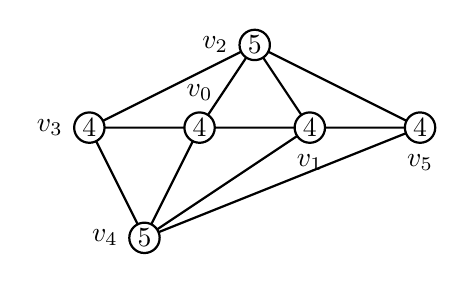
\begin{tikzpicture}[scale=0.7,
    thick,
    >=stealth',
    dot/.style = {
      draw,
      fill = white,
      circle,
      inner sep = 1pt,
      minimum size = 5pt
    }
  ]
  \coordinate (O) at (0,0);

  \draw (2,2) -- (4,2) -- (3,3.5) -- (0,2) -- (1,0) -- (6,2) -- (4,2) -- (1,0) -- (2,2) -- (0,2);
  \draw (2,2) -- (3,3.5) -- (6,2);

  \draw (2,2)       node[dot,label={above:$v_0$}] {4};
  \draw (4,2)       node[dot,label={below:$v_1$}] {4};
  \draw (3,3.5)     node[dot,label={left:$v_2$}] {5};
  \draw (0,2)       node[dot,label={left:$v_3$}] {4};
  \draw (1,0)       node[dot,label={left:$v_4$}] {5};
  \draw (6,2)       node[dot,label={below:$v_5$}] {4};
\end{tikzpicture}
\end{center}
\end{halfboxl}%
\begin{halfboxr}
\vspace{-\baselineskip}
\begin{algo}{Valence Decoding}
\textbf{Input:} An ordered list of vertex valences $[p_0, \ldots ,p_n] \in \mathbb{N}$. \\
\textbf{Output:} A triangle mesh.
\tcblower
\begin{enumerate}
    \item Create vertex $v_0$.
    \item Create $p_0$ vertices $v_1, \ldots , v_{p_0 + 1}$ (counter)clockwisely around $v_0$.
    \item Connect $v_0$ to all of these and each to its two neighbours.
    \item As long as the list isn't empty:
    \item \begin{enumerate}
        \item From $v_i$, move to $v_{i+1}$.
        \item Create $p_{i+1} - v(v_{i+1})$ further vertices (c)cw-ly.
        \item Connect them just as described above.
    \end{enumerate}
    \item Should there be a \emph{ghost vertex}, create a final vertex and connect it to all outer vertices.
\end{enumerate}
\end{algo}
\begin{center}
    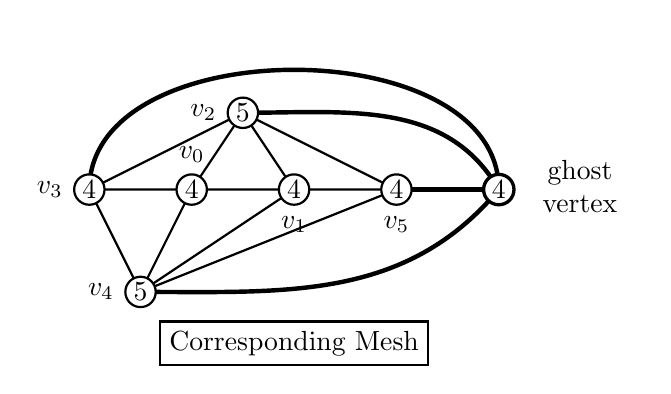
\begin{tikzpicture}[scale=0.65,
    thick,
    >=stealth',
    dot/.style = {
      draw,
      fill = white,
      circle,
      inner sep = 1pt,
      minimum size = 5pt
    }
  ]
  \coordinate (O) at (0,0);

  \draw (2,2) -- (4,2) -- (3,3.5) -- (0,2) -- (1,0) -- (6,2) -- (4,2) -- (1,0) -- (2,2) -- (0,2);
  \draw (2,2) -- (3,3.5) -- (6,2);
  \draw [ultra thick] (8,2) to[out=120,in=0] (3,3.5);
  \draw [ultra thick] (8,2) to[out=90,in=90] (0,2);
  \draw [ultra thick] (8,2) to[out=180,in=0] (6,2);
  \draw [ultra thick] (8,2) to[out=230,in=0] (1,0);

  \draw (2,2)       node[dot,label={above:$v_0$}] {4};
  \draw (4,2)       node[dot,label={below:$v_1$}] {4};
  \draw (3,3.5)     node[dot,label={left:$v_2$}] {5};
  \draw (0,2)       node[dot,label={left:$v_3$}] {4};
  \draw (1,0)       node[dot,label={left:$v_4$}] {5};
  \draw (6,2)       node[dot,label={below:$v_5$}] {4};
  \draw (8,2)       node[dot,very thick,label={right:\begin{tabular}{c}ghost  \\ vertex \end{tabular}}] {4};

  \draw (4,-1) node[rectangle, draw] {Corresponding Mesh};
\end{tikzpicture}
\end{center}
\end{halfboxr}

This is due to the ghost vertex being used to store how many vertices are located on the edges of the mesh. Thus, for example, if we stored $v_2$, we would store $p_2 = 4 + 1 = 5$, as we need to remember the ghost vertex.

\section{Constructive Solid Geometry}

In Constructive Solid Geometry (CSG), we will have the possibility of combining different objects through boolean operations. Thus, we will be describing these objects using implicit representations. In $\mathbb{R}^3$, if a point $p$ is contained by an object defined by $F: \mathbb{R}^3 \to \mathbb{R}$ if $F(p) \le 0$. Conversely, if it isn't, $F(p) > 0$ will hold.

We will consider primitives that can be given as matrix-vector products of the following form, that is, by quadratic polynomials.

$$F(x,y,z) = \begin{pmatrix} x & y & z & 1 \end{pmatrix} \cdot
\begin{pmatrix}
a & b & c & d \\
e & f & g & h \\
i & j & k & l \\
m & n & o & p
\end{pmatrix} \cdot
\begin{pmatrix} x \\ y \\ z \\ 1 \end{pmatrix}$$

\subsection{Quadrics}

\begin{halfboxl}
For quadratic polynomials, using an upper right corner matrix suffices. Preferably, symmetric matrices as described on the right may be used, as symmetric matrices have convenient properties.

\emph{Note that the matrices on the right are not equal, but their uses yield the same results for quadrics.}

In the following, we will give matrices for a few basic primitives in $\mathbb{R}^3$. These can easily be transformed into polynomials by inserting them into the formula above, for easier understanding.
\end{halfboxl}%
\begin{halfboxr}
\vspace{-\baselineskip}
\begin{defi}{Quadrics}
Quadrics are primitives in $\mathbb{R}^3$ that can be defined by polynomials of degree $2$.

They can be given as defined above using either of the following notations:
$$\begin{pmatrix}
a & b & c & d \\
0 & e & f & g \\
0 & 0 & h & i \\
0 & 0 & 0 & j
\end{pmatrix} \equiv
\begin{pmatrix}
a & \frac{b}{2} & \frac{c}{2} & \frac{d}{2} \\
\frac{b}{2} & e & \frac{f}{2} & \frac{g}{2} \\
\frac{c}{2} & \frac{f}{2} & h & \frac{i}{2} \\
\frac{d}{2} & \frac{g}{2} & \frac{i}{2} & j
\end{pmatrix}$$
\end{defi}
\end{halfboxr}

\begin{defi}{Implicit Sphere}
A sphere of radius $r$ and midpoint $m$ can be written as a quadric using the matrix
\begin{align*}Q_{sphere} &=
\begin{pmatrix}
1 & 0 & 0 & -m_x \\
0 & 1 & 0 & -m_y \\
0 & 0 & 1 & -m_z \\
-m_x & -m_y & -m_z & (m_x^2 + m_y^2 + m_z^2 - r^2)
\end{pmatrix} \\
&\equiv (x-m_x)^2 + (y-m_y)^2 + (z-m_z)^2 -r^2
\end{align*}
\end{defi}

\begin{defi}{Implicit Cylinder}
A cylinder of radius $r$, axis $(0,0,1)^T$ and going through $(m_x,m_y,0)^T$ can be written as a quadric using the matrix
\begin{align*}Q_{cylinder} &=
\begin{pmatrix}
1 & 0 & 0 & -m_x \\
0 & 1 & 0 & -m_y \\
0 & 0 & 1 & 0 \\
-m_x & -m_y & 0 & (m_x^2 + m_y^2 + - r^2)
\end{pmatrix} \\
&\equiv (x-m_x)^2 + (y-m_y)^2 - r^2
\end{align*}
\end{defi}

\begin{defi}{Implicit Cone}
A cone of apex $a$, and opening angle $\alpha$ along the $z$-axis is given by:
\begin{align*}Q_{cone} &=
\begin{pmatrix}
1 & 0 & 0 & -a_x \\
0 & 1 & 0 & -a_y \\
0 & 0 & -\tan^2 \alpha & a_z \tan^2 \alpha \\
-a_x & -a_y & a_z \tan^2 \alpha & (a_x^2 + a_y^2 - a_z^2 \tan^2 \alpha)
\end{pmatrix} \\
&\equiv (x-a_x)^2 + (y-a_y)^2 - \tan^2 \alpha (z-a_z)^2
\end{align*}
\end{defi}

\begin{halfboxl}
\vspace{-\baselineskip}
\subsection{Operations}

\subsubsection*{Transformation}

We have previously introduced transformations in the form of matrices. These also hold for CSG objects and can be applied very easily by applying the maths described on the right.
\end{halfboxl}%
\begin{halfboxr}
\vspace{-\baselineskip}
\begin{defi}{Transformation}
Given the object defined by a quadric $v^T \cdot Q \cdot v = 0$, we transform it by $M \in \mathbb{R}^{4 \times 4}$ and obtain the quadric defined by $v^T \cdot Q' \cdot v = 0$ with:
$$Q' = (M^{-1})^T \cdot Q \cdot M^{-1}$$
\end{defi}
\end{halfboxr}

\subsubsection*{Union, Intersection and Subtraction}

\begin{halfboxl}
Given two objects $F_1$ and $F_2$ given by their implicit functions, all the points lying inside them are given by $$S_i = \Set{p \in \mathbb{R}^3 : F_i(p) \le 0}, i\in \Set{1,2}.$$

With this we can intuitively and formally define the Boolean union, intersection and subtraction operations.

The union requires the point to only be contained by one of the objects. So if the minimum of the two functions is negative (implying that at least one is), then the point lies within the union.

The intersection on the other hand requires both objects to contain a point. Thus, only if the maximum of both functions is negative (implying that both are), then the point lies in the intersection.

\end{halfboxl}%
\begin{halfboxr}
\vspace{-\baselineskip}
\begin{defi}{Union}
The union of $F_1$ and $F_2$ is given by:
$$S = F(p) = \text{ min}\Set{F_1(p), F_2(p)}$$
\end{defi}

\begin{defi}{Intersection}
The intersection of $F_1$ and $F_2$ is given by:
$$S = F(p) = \text{ max}\Set{F_1(p), F_2(p)}$$
\end{defi}

\begin{defi}{Subtraction}
The subtraction of $F_1$ and $F_2$, that is, the points contained in $F_1$ but not $F_2$, is given by:
$$S = F(p) = \text{ max}\Set{F_1(p), -F_2(p)}$$
\end{defi}
\end{halfboxr}

Finally, the subtraction requires that a point be contained by $F_1$ but not $F_2$. Since the points not in $F_2$ are contained by the object $-F_2$, we can compute this as the intersection of $F_1$ and $-F_2$.

\section{Scene Representation}

\subsection{Culling}

When rendering a scene, some objects might not be fully or even at all visible for the camera. We want to render only the objects that are actually visible. We call this problem \emph{visibility determination}, and there are different approaches to solving it.

Culling is the process that allows us to avoid rendering certain faces that are not visible for the camera. We will be summarising a few of them, ordered by increasing order of computational cost.

\subsubsection*{Backface Culling}

The simplest of our techniques is backface culling. It is pretty intuitive as it simply allows removing the polygons not facing the camera, and thus assuming that all meshes are closed. Further, there are situations in which som ploygons \emph{do} face the camera but still aren't visible.

\subsubsection*{Hierarchical Frustum Culling}

Frustum culling includes backface culling, but also tests objects if they lie inside the viewing frustum. If they are inside or intersect with it, they are rendered, else they aren't.

This testing of objects can be excessively expensive for complex objects, thus it is often faster, though less accurate, to construct bounding boxes around objects and testing the boxes.

We now introduce three types of boxes, sorted by decreasing included empty space and increasing intersection test costs.

The \emph{bounding sphere} simply constructs a sphere around the object. The \emph{axis-aligned bounding box} constructs a box around the object while keeping it aligned to the axes (duh!). Similarly obvious is the \emph{oriented bounding box} which creates the box of smallest volume around an object.

The hierarchical part comes in by creating bounding boxes around bounding boxes. If such a bounding box is fully in- or outside, so are all the children. If it's an intersection, we test the children individually.

\subsubsection*{Portal Culling}

\emph{Portal culling} applies frustum culling, then works with high level knowledge of a scene and divides architectural scenes in rooms connected by portals. Then we use the frustum to detect the visible portals and recursively generate further, smaller frustums and cull further. This can become difficult if reflective surfaces are present.

\subsubsection*{Occlusion Culling}

\emph{Occlusion culling} renders objects front to back, while keeping track of rendered objects as occluders. If, for an object, less than a given amount of fragments $n$ (Level Of Detail, LOD) are visible because the rest are covered by occluders, we do not render said object (because if we did, the tests would take forever and be pretty much useless).

\subsection{Optimisation structures}

\subsubsection*{Quad/Octrees}

\begin{halfboxl}
Remember \emph{Binary Trees}, also called Bintrees? Well, \textit{Quadtrees} and \textit{Octrees} are pretty similar in principle, except that you use them to split $2$ and $3$ dimensional space respectively.

Take a square. You can divide it into four smaller, equally sized squares. Similarly, a cube can be divided into 8 equally sized cubes.

On the right you see a quadtree, but it should by now be pretty obvious what an octree would look like.
\end{halfboxl}%
\begin{halfboxr}
\vspace{-\baselineskip}
\begin{center}
    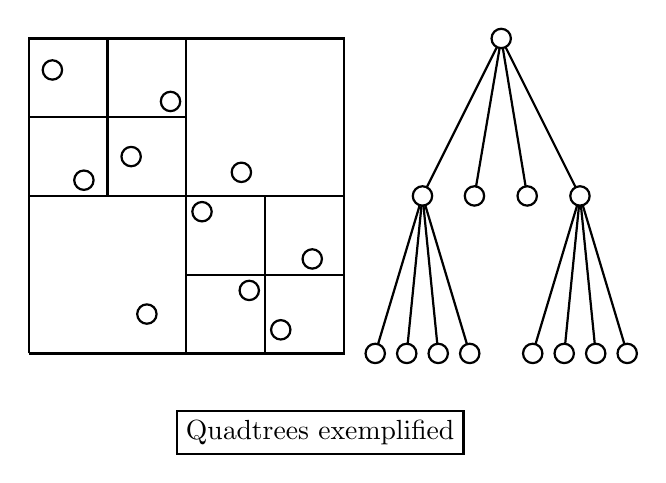
\begin{tikzpicture}[
    thick,
    >=stealth',
    dot/.style = {
      draw,
      fill = white,
      circle,
      inner sep = 0pt,
      minimum size = 7pt
    }
  ]
  \coordinate (O) at (0,0);

  \draw (0,0) -- (0,4) -- (4,4) -- (4,0) -- (0,0);

  \draw (2,0) -- (2,4);
  \draw (0,2) -- (4,2);

  \draw (1,2) -- (1,4);
  \draw (0,3) -- (2,3);

  \draw (3,0) -- (3,2);
  \draw (2,1) -- (4,1);

  \draw (6,4) -> (5,2);
  \draw (6,4) -> (5.66,2);
  \draw (6,4) -> (6.33,2);
  \draw (6,4) -> (7,2);

  \draw (5,2) -> (4.4,0);
  \draw (5,2) -> (4.8,0);
  \draw (5,2) -> (5.2,0);
  \draw (5,2) -> (5.6,0);

  \draw (7,2) -> (6.4,0);
  \draw (7,2) -> (6.8,0);
  \draw (7,2) -> (7.2,0);
  \draw (7,2) -> (7.6,0);


  \draw (6,4)   node[dot]   {};
  \draw (5.66,2)   node[dot]   {};
  \draw (5,2)   node[dot]   {};
  \draw (6.33,2)   node[dot]   {};
  \draw (7,2)   node[dot]   {};

  \draw (4.4,0)   node[dot]   {};
  \draw (4.8,0)   node[dot]   {};
  \draw (5.2,0)   node[dot]   {};
  \draw (5.6,0)   node[dot]   {};

  \draw (6.4,0)   node[dot]   {};
  \draw (6.8,0)   node[dot]   {};
  \draw (7.2,0)   node[dot]   {};
  \draw (7.6,0)   node[dot]   {};

  \draw (1.5,0.5)   node[dot]   {};
  \draw (0.3,3.6)   node[dot]   {};
  \draw (0.7,2.2)   node[dot]   {};
  \draw (1.8,3.2)   node[dot]   {};
  \draw (1.3,2.5)   node[dot]   {};

  \draw (2.7,2.3)   node[dot]   {};
  \draw (2.2,1.8)   node[dot]   {};
  \draw (2.8,0.8)   node[dot]   {};
  \draw (3.6,1.2)   node[dot]   {};
  \draw (3.2,0.3)   node[dot]   {};

  \draw (3.7,-1) node[rectangle, draw] {Quadtrees exemplified};
\end{tikzpicture}
\end{center}
\end{halfboxr}

\subsubsection*{KD Trees}

\begin{halfboxl}
Now, we saw that quadtrees aren't very apt at splitting scenes into balanced subdivisions. That's why we are going to introduce \emph{KD trees}.

Contrary to quadtrees these are not independent of the scene, but they are capable of dividing it into more or less equal parts by splitting horizontally and vertically not at the centres, but rather where it actually makes sense.

However, we still split horizontally, then vertically, then horizontally and so on.
\end{halfboxl}%
\begin{halfboxr}
\vspace{-\baselineskip}
\begin{center}
    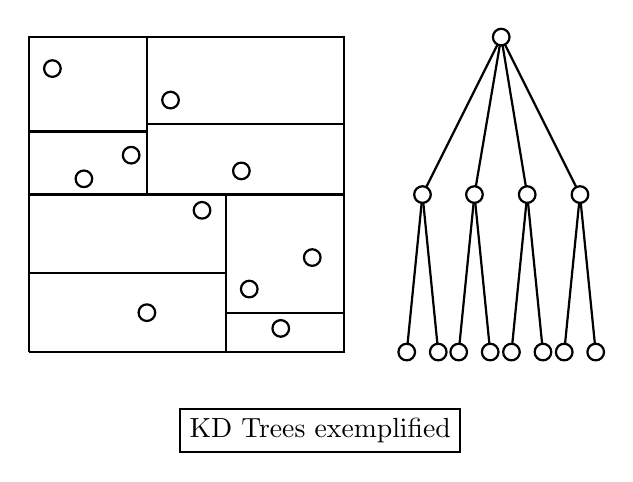
\begin{tikzpicture}[
    thick,
    >=stealth',
    dot/.style = {
      draw,
      fill = white,
      circle,
      inner sep = 0pt,
      minimum size = 6pt
    }
  ]
  \coordinate (O) at (0,0);

  \draw (0,0) -- (0,4) -- (4,4) -- (4,0) -- (0,0);

  \draw (0,2) -- (4,2);

  \draw (2.5,0) -- (2.5,2);
  \draw (1.5,2) -- (1.5,4);

  \draw (0,1) -- (2.5,1);
  \draw (2.5,0.5) -- (4,0.5);
  \draw (0,2.8) -- (1.5,2.8);
  \draw (1.5,2.9) -- (4,2.9);


  \draw (6,4) -> (5,2);
  \draw (6,4) -> (5.66,2);
  \draw (6,4) -> (6.33,2);
  \draw (6,4) -> (7,2);

  \draw (5,2) -> (4.8,0);
  \draw (5,2) -> (5.2,0);

  \draw (5.66,2) -> (5.46,0);
  \draw (5.66,2) -> (5.86,0);

  \draw (6.33,2) -> (6.13,0);
  \draw (6.33,2) -> (6.53,0);

  \draw (7,2) -> (6.8,0);
  \draw (7,2) -> (7.2,0);



  \draw (6,4)   node[dot]   {};
  \draw (5.66,2)   node[dot]   {};
  \draw (5,2)   node[dot]   {};
  \draw (6.33,2)   node[dot]   {};
  \draw (7,2)   node[dot]   {};

  \draw (4.8,0)   node[dot]   {};
  \draw (5.2,0)   node[dot]   {};
  \draw (5.46,0)   node[dot]   {};
  \draw (5.86,0)   node[dot]   {};

  \draw (6.13,0)   node[dot]   {};
  \draw (6.53,0)   node[dot]   {};
  \draw (6.8,0)   node[dot]   {};
  \draw (7.2,0)   node[dot]   {};

  \draw (1.5,0.5)   node[dot]   {};
  \draw (0.3,3.6)   node[dot]   {};
  \draw (0.7,2.2)   node[dot]   {};
  \draw (1.8,3.2)   node[dot]   {};
  \draw (1.3,2.5)   node[dot]   {};

  \draw (2.7,2.3)   node[dot]   {};
  \draw (2.2,1.8)   node[dot]   {};
  \draw (2.8,0.8)   node[dot]   {};
  \draw (3.6,1.2)   node[dot]   {};
  \draw (3.2,0.3)   node[dot]   {};

  \draw (3.7,-1) node[rectangle, draw] {KD Trees exemplified};
\end{tikzpicture}
\end{center}
\end{halfboxr}

\subsubsection*{Binary Space Partitioning}

\textit{Binary Space Partitioning} (BSP) is just a further generalisation of KD Trees where we don't even split horizontally or vertically, but only how it best suits us to further balance our tree.

We will not illustrate this concept at this point because we're too lazy to create the corresponding diagram. However, as a reader, picture BSP as a diagram of a KD tree in which all lines, instead of being all nice and perpendicular to each other, are skewed and diagonal and do not satisfy your inner OCD at all.

\section{Volumetric Rendering}

\subsection{Signed Distance Function}

\begin{halfboxl}
A \emph{Signed Distance Function} is a special case of an implicit function in that it also returns the \emph{sign} between a point and the object. It of course keeps the \emph{sign}, positive if outside, negative if inside. The name should now seem well chosen.
\end{halfboxl}%
\begin{halfboxr}
\vspace{-\baselineskip}
\begin{defi}{Signed Distance Function}
\[F(x) = \text{min}_{p \in S} ||p - x|| \cdot \begin{cases} +1 \quad \text{if } x \text{ outside} \\ -1 \quad \text{else} \end{cases}\]
\end{defi}
\end{halfboxr}

Another concept are \emph{Value Functions} which attribute, to any point in space, a value corresponding to a property, e.g. temperature, density etc. From such functions, we can generate sets of points with the same property, creating surfaces which we call \emph{iso-surfaces}.

\begin{halfboxl}
An example for these are CT or MRT Scans, which use tissue density as a function to specify differing surfaces. This means that in practice, we won't have continuous functions, but discrete samples which, we will assume w.l.o.g., are given for a regular 3D grid with distances of $1$.

The technique we will be using is similar to bilinear interpolation and called \emph{trilinear interpolation}. Given how our grid is defined, we can consider it as a bunch of cubes, each specified by eight measurement points.
\end{halfboxl}%
\begin{halfboxr}
\vspace{-\baselineskip}
\begin{align*}
F(x,y,z)=   & \quad F_{0,0,0} \cdot (1-x)(1-y)(1-z)\\
            & + F_{1,0,0}\cdot x(1-y)(1-z)\\
            & + F_{0,1,0}\cdot (1-x)y(1-z)\\
            & + F_{1,1,0}\cdot xy(1-z)\\
            & + F_{0,0,1}\cdot (1-x)(1-y)z\\
            & + F_{1,0,1}\cdot x(1-y)z\\
            & + F_{0,1,1}\cdot (1-x)yz\\
            & + F_{1,1,1}\cdot xyz\\
\end{align*}
\end{halfboxr}
Thus, for a point located within such a cube, we can approximate its value function by interpolating it using these eight points $F_{a,b,c}, \enskip a,b,c \in \Set{0,1}$.

\subsection{Direct Volume Rendering}

Given a volumetric scene, we can use \emph{ray casting} to determine the colour of a pixel by casting a ray for each pixel and adding the colours and opacities of the different layers.

For this, there are two approaches: Front-to-back ray casting and back-to-front ray casting. In the following $c_i$ represents the colour of the $i$th layer, $\alpha_i$ its opacity and $\hat c_i = \alpha_i c_i$ its opacity-weighted colour with $i \in \Set{0,...,k}$. We assume that $c_i$ and $\alpha_i$ are values in $[0,1]$.

\begin{halfboxl}
\vspace{-\baselineskip}
\begin{defi}{Front-to-Back}
With $\hat C_0 = \hat c_0$ and $A_0 = \alpha_0$, we apply

$$\hat C_i = \hat C_{i-1} + (1 - A_{i-1}) \hat c_i$$
$$A_i = A_{i-1} + (1 - A_{i-1}) \alpha_i$$

recursively until $i = k$ or until $A_i = 1$, that is, when we have reached total opacity.
\end{defi}
\end{halfboxl}%
\begin{halfboxr}
\vspace{-\baselineskip}
\begin{defi}{Back-to-Front}
Let $\hat C_k = \hat c_k$. Then, with

$$\hat C_i = \hat c_i + (1 - \hat \alpha) \hat C_{i+1}$$

the final opacity-weighted colour is $\hat C_0$.
\end{defi}
\end{halfboxr}

\subsection{Indirect Volume Rendering}


\begin{halfboxl}
For indirect volume rendering, we use the \emph{Marching Cubes} algorithm. To make it simple, we discretely sample our scene with a three-dimensional grid, measuring a certain metric. This allows us to create a signed distance function, from which we can compute a mesh.

We will illustrate it using a simplified algorithm, that is, the marching \emph{squares} algorithm.

As the function is a signed distance function, points with negative value lie within the polygon, while points with positive values lie outside. And the distance part allows us to compare the ratios between the points to approximate more precisely how the polygon is shaped.

However, the dotted lines in our example are problematic, as both the displayed polygon shapes are valid interpretations. There are two common solutions to this issue. Either, we assume the sign of the centre of any square to be positive or negative, which we can always do, or we do a further measurement whenever there is more than one possibility, which depends on the use case.

Note that this method can be imprecise and prone to aliasing, as it may cut off, for example, entire triangles contained in a single square. There are many sampling methods to make this more precise.
\end{halfboxl}%
\begin{halfboxr}
\vspace{-\baselineskip}
\begin{center}
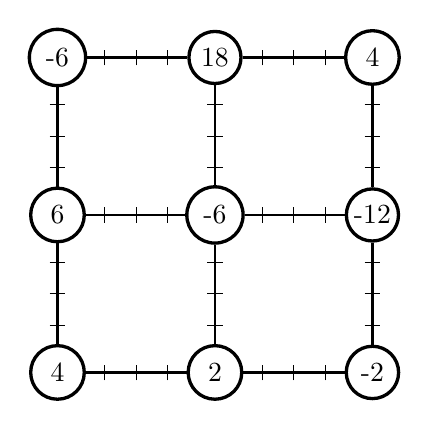
\begin{tikzpicture}{1}
\begin{scope}[every node/.style={circle,thick,draw, inner sep = 4pt}]
    \draw (0.6,-0.1) -- (0.6,0.1);
    \draw (1,-0.1) -- (1,0.1);
    \draw (1.4,-0.1) -- (1.4,0.1);

    \draw (0.6,1.9) -- (0.6,2.1);
    \draw (1,1.9) -- (1,2.1);
    \draw (1.4,1.9) -- (1.4,2.1);

    \draw (0.6,3.9) -- (0.6,4.1);
    \draw (1,3.9) -- (1,4.1);
    \draw (1.4,3.9) -- (1.4,4.1);

    \draw (2.6,-0.1) -- (2.6,0.1);
    \draw (3,-0.1) -- (3,0.1);
    \draw (3.4,-0.1) -- (3.4,0.1);

    \draw (2.6,1.9) -- (2.6,2.1);
    \draw (3,1.9) -- (3,2.1);
    \draw (3.4,1.9) -- (3.4,2.1);

    \draw (2.6,3.9) -- (2.6,4.1);
    \draw (3,3.9) -- (3,4.1);
    \draw (3.4,3.9) -- (3.4,4.1);

    \draw (-0.1,0.6) -- (0.1,0.6);
    \draw (-0.1,1) -- (0.1,1);
    \draw (-0.1,1.4) -- (0.1,1.4);

    \draw (1.9,0.6) -- (2.1,0.6);
    \draw (1.9,1) -- (2.1,1);
    \draw (1.9,1.4) -- (2.1,1.4);

    \draw (3.9,0.6) -- (4.1,0.6);
    \draw (3.9,1) -- (4.1,1);
    \draw (3.9,1.4) -- (4.1,1.4);

    \draw (-0.1,2.6) -- (0.1,2.6);
    \draw (-0.1,3) -- (0.1,3);
    \draw (-0.1,3.4) -- (0.1,3.4);

    \draw (1.9,2.6) -- (2.1,2.6);
    \draw (1.9,3) -- (2.1,3);
    \draw (1.9,3.4) -- (2.1,3.4);

    \draw (3.9,2.6) -- (4.1,2.6);
    \draw (3.9,3) -- (4.1,3);
    \draw (3.9,3.4) -- (4.1,3.4);

    \node [very thick] (a) at (0,0) {4};
    \node [very thick] (b) at (2,0) {2};
    \node [very thick, inner sep = 3] (c) at (4,0) {-2};
    \node [very thick] (d) at (0,2) {6};
    \node [very thick, inner sep = 3.5] (e) at (2,2) {-6};
    \node [very thick, inner sep = 1.5] (f) at (4,2) {-12};
    \node [very thick, inner sep = 3.5] (g) at (0,4) {-6};
    \node [very thick, inner sep = 2.5] (h) at (2,4) {18};
    \node [very thick] (i) at (4,4) {4};

    \path [thick] (a) edge (b);
    \path [thick] (a) edge (d);
    \path [thick] (b) edge (c);
    \path [thick] (b) edge (e);
    \path [thick] (c) edge (f);
    \path [thick] (d) edge (g);
    \path [thick] (d) edge (e);
    \path [thick] (e) edge (h);
    \path [thick] (e) edge (f);
    \path [thick] (f) edge (i);
    \path [thick] (g) edge (h);
    \path [thick] (h) edge (i);

\end{scope}

\end{tikzpicture}
\end{center}


\begin{center}
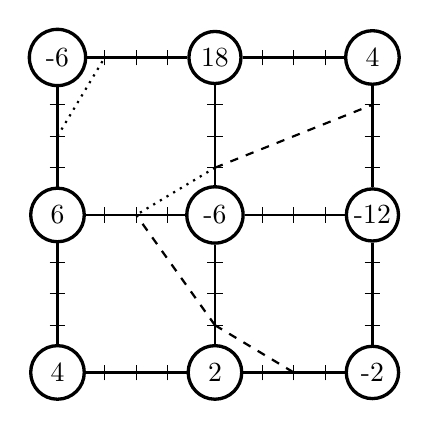
\begin{tikzpicture}{1}
\begin{scope}[every node/.style={circle,thick,draw, inner sep = 4pt}]
    \draw (0.6,-0.1) -- (0.6,0.1);
    \draw (1,-0.1) -- (1,0.1);
    \draw (1.4,-0.1) -- (1.4,0.1);

    \draw (0.6,1.9) -- (0.6,2.1);
    \draw (1,1.9) -- (1,2.1);
    \draw (1.4,1.9) -- (1.4,2.1);

    \draw (0.6,3.9) -- (0.6,4.1);
    \draw (1,3.9) -- (1,4.1);
    \draw (1.4,3.9) -- (1.4,4.1);

    \draw (2.6,-0.1) -- (2.6,0.1);
    \draw (3,-0.1) -- (3,0.1);
    \draw (3.4,-0.1) -- (3.4,0.1);

    \draw (2.6,1.9) -- (2.6,2.1);
    \draw (3,1.9) -- (3,2.1);
    \draw (3.4,1.9) -- (3.4,2.1);

    \draw (2.6,3.9) -- (2.6,4.1);
    \draw (3,3.9) -- (3,4.1);
    \draw (3.4,3.9) -- (3.4,4.1);

    \draw (-0.1,0.6) -- (0.1,0.6);
    \draw (-0.1,1) -- (0.1,1);
    \draw (-0.1,1.4) -- (0.1,1.4);

    \draw (1.9,0.6) -- (2.1,0.6);
    \draw (1.9,1) -- (2.1,1);
    \draw (1.9,1.4) -- (2.1,1.4);

    \draw (3.9,0.6) -- (4.1,0.6);
    \draw (3.9,1) -- (4.1,1);
    \draw (3.9,1.4) -- (4.1,1.4);

    \draw (-0.1,2.6) -- (0.1,2.6);
    \draw (-0.1,3) -- (0.1,3);
    \draw (-0.1,3.4) -- (0.1,3.4);

    \draw (1.9,2.6) -- (2.1,2.6);
    \draw (1.9,3) -- (2.1,3);
    \draw (1.9,3.4) -- (2.1,3.4);

    \draw (3.9,2.6) -- (4.1,2.6);
    \draw (3.9,3) -- (4.1,3);
    \draw (3.9,3.4) -- (4.1,3.4);

    \node [very thick] (a) at (0,0) {4};
    \node [very thick] (b) at (2,0) {2};
    \node [very thick, inner sep = 3] (c) at (4,0) {-2};
    \node [very thick] (d) at (0,2) {6};
    \node [very thick, inner sep = 3.5] (e) at (2,2) {-6};
    \node [very thick, inner sep = 1.5] (f) at (4,2) {-12};
    \node [very thick, inner sep = 3.5] (g) at (0,4) {-6};
    \node [very thick, inner sep = 2.5] (h) at (2,4) {18};
    \node [very thick] (i) at (4,4) {4};

    \path [thick] (a) edge (b);
    \path [thick] (a) edge (d);
    \path [thick] (b) edge (c);
    \path [thick] (b) edge (e);
    \path [thick] (c) edge (f);
    \path [thick] (d) edge (g);
    \path [thick] (d) edge (e);
    \path [thick] (e) edge (h);
    \path [thick] (e) edge (f);
    \path [thick] (f) edge (i);
    \path [thick] (g) edge (h);
    \path [thick] (h) edge (i);

    \draw [dashed,thick] (2,0.6) -- (3,0);
    \draw [dashed,thick] (2,0.6) -- (1,2);
    \draw [dotted,thick] (2,2.6) -- (1,2);
    \draw [dashed,thick] (2,2.6) -- (4,3.4);
    \draw [dotted,thick] (0,3) -- (0.6,4);

\end{scope}

\end{tikzpicture}
\end{center}


\begin{center}
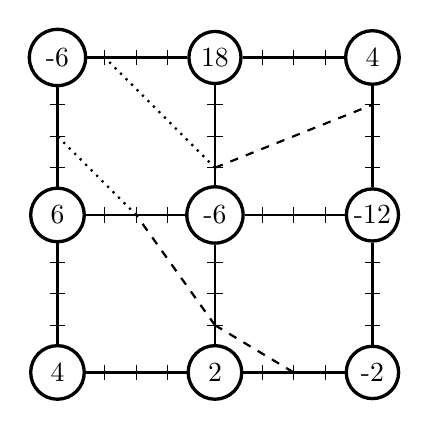
\begin{tikzpicture}{1}
\begin{scope}[every node/.style={circle,thick,draw, inner sep = 4pt}]
    \draw (0.6,-0.1) -- (0.6,0.1);
    \draw (1,-0.1) -- (1,0.1);
    \draw (1.4,-0.1) -- (1.4,0.1);

    \draw (0.6,1.9) -- (0.6,2.1);
    \draw (1,1.9) -- (1,2.1);
    \draw (1.4,1.9) -- (1.4,2.1);

    \draw (0.6,3.9) -- (0.6,4.1);
    \draw (1,3.9) -- (1,4.1);
    \draw (1.4,3.9) -- (1.4,4.1);

    \draw (2.6,-0.1) -- (2.6,0.1);
    \draw (3,-0.1) -- (3,0.1);
    \draw (3.4,-0.1) -- (3.4,0.1);

    \draw (2.6,1.9) -- (2.6,2.1);
    \draw (3,1.9) -- (3,2.1);
    \draw (3.4,1.9) -- (3.4,2.1);

    \draw (2.6,3.9) -- (2.6,4.1);
    \draw (3,3.9) -- (3,4.1);
    \draw (3.4,3.9) -- (3.4,4.1);

    \draw (-0.1,0.6) -- (0.1,0.6);
    \draw (-0.1,1) -- (0.1,1);
    \draw (-0.1,1.4) -- (0.1,1.4);

    \draw (1.9,0.6) -- (2.1,0.6);
    \draw (1.9,1) -- (2.1,1);
    \draw (1.9,1.4) -- (2.1,1.4);

    \draw (3.9,0.6) -- (4.1,0.6);
    \draw (3.9,1) -- (4.1,1);
    \draw (3.9,1.4) -- (4.1,1.4);

    \draw (-0.1,2.6) -- (0.1,2.6);
    \draw (-0.1,3) -- (0.1,3);
    \draw (-0.1,3.4) -- (0.1,3.4);

    \draw (1.9,2.6) -- (2.1,2.6);
    \draw (1.9,3) -- (2.1,3);
    \draw (1.9,3.4) -- (2.1,3.4);

    \draw (3.9,2.6) -- (4.1,2.6);
    \draw (3.9,3) -- (4.1,3);
    \draw (3.9,3.4) -- (4.1,3.4);

    \node [very thick] (a) at (0,0) {4};
    \node [very thick] (b) at (2,0) {2};
    \node [very thick, inner sep = 3] (c) at (4,0) {-2};
    \node [very thick] (d) at (0,2) {6};
    \node [very thick, inner sep = 3.5] (e) at (2,2) {-6};
    \node [very thick, inner sep = 1.5] (f) at (4,2) {-12};
    \node [very thick, inner sep = 3.5] (g) at (0,4) {-6};
    \node [very thick, inner sep = 2.5] (h) at (2,4) {18};
    \node [very thick] (i) at (4,4) {4};

    \path [thick] (a) edge (b);
    \path [thick] (a) edge (d);
    \path [thick] (b) edge (c);
    \path [thick] (b) edge (e);
    \path [thick] (c) edge (f);
    \path [thick] (d) edge (g);
    \path [thick] (d) edge (e);
    \path [thick] (e) edge (h);
    \path [thick] (e) edge (f);
    \path [thick] (f) edge (i);
    \path [thick] (g) edge (h);
    \path [thick] (h) edge (i);

    \draw [dashed,thick] (2,0.6) -- (3,0);
    \draw [dashed,thick] (2,0.6) -- (1,2);
    \draw [dotted,thick] (1,2) -- (0,3);
    \draw [dashed,thick] (2,2.6) -- (4,3.4);
    \draw [dotted,thick] (2,2.6) -- (0.6,4);

\end{scope}

\end{tikzpicture}
\end{center}

\end{halfboxr}

\section{Curves}

In this chapter, unlike in the lecture, we will not go into the formal aspects of the subject as this would exceed the scope of what we are trying to achieve. However, we highly recommend you check it out in the lecture, as it is important for a good understanding of the substance.

\begin{halfboxl}
\vspace{-\baselineskip}

\subsection{Bézier Curves}

A \emph{Bézier curve} given by $n+1$ control points is the curve given by a polynomial of degree $n$. As such, the curve on the right, which is specified by $4$ control points, is of degree $3$.

\subsection{De Casteljau Algorithm}

The \emph{De Casteljau algorithm} allows us to discretise a given Bézier curve with an arbitrarily high precision by evaluating the polynomial for any amount of parameters $t \in [0,1]$. Its application is, somewhat poorly, visualised on the right.

\subsection{Bézier Spline}

A \emph{Bézier Spline}, or composite Bézier curve is a curve made up of multiple Bézier curves which are, in applications, usually of degree $3$. This guarantees a high stability, as opposed to a single, high degree curve.

Given a set of points $4$ control points and a further set of points we want to interpolate, we can use the \emph{A-Frame construction} to create further control points that create a Bézier spline through these points.

On the right, we are given $a_i, \enskip i \in \Set{0,1,2,3}$ and $B$. Then, the dotted lines and the $A$s are our A-frame elements while the dashed segments along with $b_i, \enskip i \in \Set{0,1,2,3}$, with $a_3 = b_0$ and $b_3 = B$ the next interpolated Bézier curve.

The A-Frame construction tells us that $[a_1,a_2] = [a_2,A_{\alpha}]$, that $[A_{\alpha},a_3] = [b_0,b_1] = [b_1,A_{\beta}]$ and that $[A_{\beta},b_2] = [b_2,b_3]$.
\end{halfboxl}%
\begin{halfboxr}
\vspace{-\baselineskip}
\begin{center}
    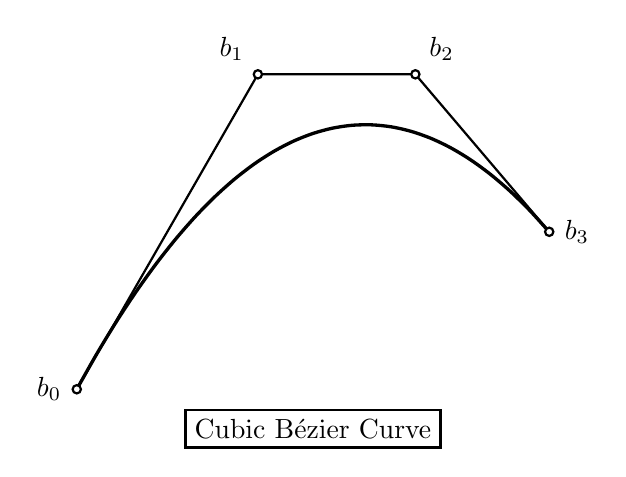
\begin{tikzpicture}[
    thick,
    >=stealth',
    dot/.style = {
      draw,
      fill = white,
      circle,
      inner sep = 0pt,
      minimum size = 3pt
    }
  ]
  \coordinate (O) at (0,0);

  \draw[scale=1,domain=0:6,smooth,variable=\x,black,very thick] plot ({\x},{-0.25*\x*\x + 1.833*\x});

  \draw (0,0) -- (2.3,4) -- (4.3,4) -- (6,2);

  \draw (0,0)   node[dot,label={left:$b_0$}]    {};
  \draw (2.3,4)   node[dot,label={above left:$b_1$}]   {};
  \draw (4.3,4)   node[dot,label={above right:$b_2$}]   {};
  \draw (6,2)   node[dot,label={right:$b_3$}]   {};

  \draw (3,-0.5) node[rectangle, draw] {Cubic Bézier Curve};
\end{tikzpicture}
\end{center}

\begin{center}
    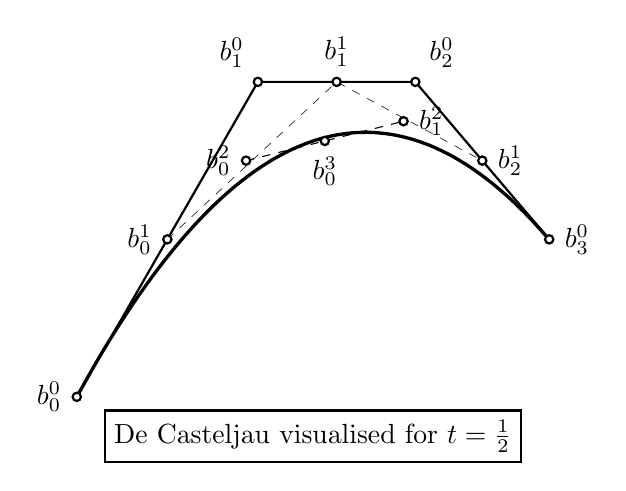
\begin{tikzpicture}[
    thick,
    >=stealth',
    dot/.style = {
      draw,
      fill = white,
      circle,
      inner sep = 0pt,
      minimum size = 3pt
    }
  ]
  \coordinate (O) at (0,0);

  \draw[scale=1,domain=0:6,smooth,variable=\x,black,very thick] plot ({\x},{-0.25*\x*\x + 1.833*\x});

  \draw (0,0) -- (2.3,4) -- (4.3,4) -- (6,2);

  \draw (0,0)   node[dot,label={left:$b_0^0$}]    {};
  \draw (2.3,4)   node[dot,label={above left:$b_1^0$}]   {};
  \draw (4.3,4)   node[dot,label={above right:$b_2^0$}]   {};
  \draw (6,2)   node[dot,label={right:$b_3^0$}]   {};

  \draw [very thin,dashed] (1.15,2) -- (3.3,4) -- (5.15,3);
  \draw [thin,dashed] (2.15,3) -- (4.15,3.5);

  \draw (1.15,2) node[dot,label={left:$b_0^1$}]    {};
  \draw (3.3,4) node[dot,label={above:$b_1^1$}]   {};
  \draw (5.15,3) node[dot,label={right:$b_2^1$}]   {};

  \draw (2.15,3)   node[dot,label={left:$b_0^2$}]    {};
  \draw (4.15,3.5) node[dot,label={right:$b_1^2$}]    {};

  \draw (3.15,3.25) node[dot,label={below:$b_0^3$}]    {};

  \draw (3,-0.5) node[rectangle, draw] {De Casteljau visualised for $t=\frac{1}{2}$};
\end{tikzpicture}
\end{center}

\begin{center}
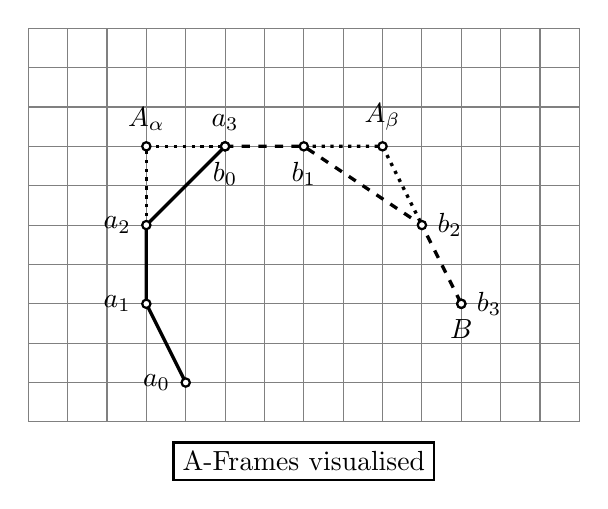
\begin{tikzpicture}[
    thick,
    >=stealth',
    dot/.style = {
      draw,
      fill = white,
      circle,
      inner sep = 0pt,
      minimum size = 3pt
    }
  ]
% grid
\draw[thin,black!50]   (0,0) grid[step= 5mm] ++ (7,5);

\draw[very thick] (2,.5) -- (1.5,1.5) -- (1.5,2.5) -- (2.5,3.5);
\draw[very thick,dotted] (1.5,2.5) -- (1.5,3.5) -- (2.5,3.5);
\draw[very thick,dashed] (2.5,3.5) -- (3.5,3.5) -- (5,2.5) -- (5.5,1.5);
\draw[very thick,dotted] (3.5,3.5) -- (4.5,3.5) -- (5,2.5);

% axis
% curve


  \draw (2,.5)   node[dot,label={left:$a_0$}]    {};
  \draw (1.5,1.5)   node[dot,label={left:$a_1$}]    {};
  \draw (1.5,2.5)   node[dot,label={left:$a_2$}]    {};
  \draw (2.5,3.5)   node[dot,label={above:$a_3$}]    {};
  \draw (2.5,3.5)   node[dot,label={below:$b_0$}]    {};
  \draw (3.5,3.5)   node[dot,label={below:$b_1$}]    {};
  \draw (5,2.5)   node[dot,label={right:$b_2$}]    {};
  \draw (5.5,1.5)   node[dot,label={right:$b_3$}]    {};
  \draw (5.5,1.5)   node[dot,label={below:$B$}]    {};

  \draw (1.5,3.5)   node[dot,label={above:$A_{\alpha}$}]    {};
  \draw (4.5,3.5)   node[dot,label={above:$A_{\beta}$}]    {};

  \draw (3.5,-0.5) node[rectangle, draw] {A-Frames visualised};

\end{tikzpicture}
\end{center}
\end{halfboxr}

As an addition to the lecture, we recommend you create a few examples of these concepts and complete them graphically on your own as to get an intuitive feel for them.

\end{document}
